\documentclass[12pt,english,british]{article}
%DIF LATEXDIFF DIFFERENCE FILE
%DIF DEL full_article_old.tex   Mon Nov 23 16:27:01 2015
%DIF ADD full_article.tex       Mon Nov 23 18:28:33 2015
\usepackage[affil-it]{authblk}
\usepackage{graphicx}
\usepackage[space]{grffile}
\usepackage{latexsym}
\usepackage{textcomp}
\usepackage{longtable}
\usepackage{multirow,booktabs}
\usepackage{amsfonts,amsmath,amssymb}
\usepackage{url}
%\usepackage[utf8]{inputenc}
\usepackage{hyperref}
\hypersetup{colorlinks=false,pdfborder={0 0 0}}
%\usepackage{latexml}
\newcommand{\truncateit}[1]{\truncate{0.8\textwidth}{#1}}
\newcommand{\scititle}[1]{\title[\truncateit{#1}]{#1}}

\usepackage{lmodern}
\usepackage[T1]{fontenc}
\usepackage[latin9]{inputenc}
\usepackage{geometry}
\geometry{verbose,tmargin=2.5cm,bmargin=2.5cm,lmargin=3cm,rmargin=2.5cm}
\providecommand{\tabularnewline}{\\}
\usepackage[nolist]{acronym}
\newacro{BMI} {body mass index}  
\newacro{LMICs} {low- and middle-income countries}  
\newacro{LMIC} {low- and middle-income country}  
\newacro{MICs} {middle-income countries} 
\newacro{HICs} {high-income countries} 
\newacro{MIC} {middle-income country}  
\newacro{HIC} {high-income country}  
 \newacro{FE} {fixed effects}  
\newacro{HbA1c} {glycated hemoglobin}  
\newacro{IDF} {International Diabetes Federation}  
\newacro{IV} {instrumental variable}  
\newacro{MxFLS} {Mexican Family Life Survey}  
\newacro{OLS} {ordinary least squares}  
\newacro{RE} {random effects}  
\newacro{T2DM} {Type II Diabetes mellitus}  
\newacro{US} {United States}
\newacro{WHO} {World Health Organization} 
\newacro{USA} {United States of America}   
\usepackage{longtable}
\usepackage{booktabs}
%\usepackage{dcolumn}
% Added by lyx2lyx
\usepackage{multirow}
\usepackage{graphicx}
\usepackage[Export]{adjustbox}
%\newcommand{\sym}[1]{\ensuremath{^{#1}}} % for symbols in Table
\usepackage{pdflscape}
\usepackage[authoryear]{natbib}


% paper margins
\usepackage{geometry}
\geometry{
letterpaper,
left=25mm,
right=30mm,
top=20mm,
bottom=30mm,
}   
%limiting tables to only float within section
\usepackage[section]{placeins}
  
%use for commands only working with pdf
  
% formatation

\usepackage{listings}
\lstset{ %
  backgroundcolor=\color{white},   % choose the background color
  basicstyle=\footnotesize,        % size of fonts used for the code
  breaklines=true,                 % automatic line breaking only at whitespace
  captionpos=b,                    % sets the caption-position to bottom
  commentstyle=\color{OliveGreen},    % comment style
  keywordstyle=\color{BlueViolet},       % keyword style
  stringstyle=\color{black},     % string literal style
  language=[AlLaTeX]TeX,             % Set your language (you can change the language for each code-block optionally)
  frame=lrtb, %
  xleftmargin=\fboxsep, %
  xrightmargin=-\fboxsep, %
  moretexcs={lstset,color,colorlet, cellcolor, newcolumntype, columncolor, rowcolor, multirow, xspace, LaTeX, TeX},
}
% *****************************************************************
% Estout related things
% *****************************************************************
\newcommand{\sym}[1]{\rlap{#1}}% Thanks to David Carlisle

\let\estinput=\input% define a new input command so that we can still flatten the document

\newcommand{\estwide}[3]{
		\vspace{.75ex}{
			\begin{tabular*}
			{\textwidth}{@{\hskip\tabcolsep\extracolsep\fill}l*{#2}{#3}}
			\toprule
			\estinput{#1}
			\bottomrule
			\addlinespace[.75ex]
			\end{tabular*}
			}
		}	

\newcommand{\estauto}[3]{
		\vspace{.75ex}{
			\begin{tabular}{l*{#2}{#3}}
			\toprule
			\estinput{#1}
			\bottomrule
			\addlinespace[.75ex]
			\end{tabular}
			}
		}

% Allow line breaks with \\ in specialcells
	\newcommand{\specialcell}[2][c]{%
	\begin{tabular}[#1]{@{}c@{}}#2\end{tabular}}

% *****************************************************************
% Custom subcaptions
% *****************************************************************
% Note/Source/Text after Tables
\newcommand{\figtext}[1]{
	\vspace{-1.9ex}
	\captionsetup{justification=justified,font=footnotesize}
	\caption*{\hspace{6pt}\hangindent=1.5em #1}
	}
\newcommand{\fignote}[1]{\figtext{\emph{Note:~}~#1}}

\newcommand{\figsource}[1]{\figtext{\emph{Source:~}~#1}}

% Add significance note with \starnote
\newcommand{\starnote}{\figtext{* p < 0.1, ** p < 0.05, *** p < 0.01. Robust standard errors in parentheses.}}

% *****************************************************************
% siunitx
% *****************************************************************
\usepackage{siunitx} % centering in tables
	\sisetup{
		detect-mode,
		tight-spacing		= true,
		group-digits		= false ,
		input-signs		= ,
		input-symbols		= ( ) [ ] - + *,
		input-open-uncertainty	= ,
		input-close-uncertainty	= ,
		table-align-text-post	= false
        }
%DIF PREAMBLE EXTENSION ADDED BY LATEXDIFF
%DIF UNDERLINE PREAMBLE %DIF PREAMBLE
\RequirePackage[normalem]{ulem} %DIF PREAMBLE
\RequirePackage{color}\definecolor{RED}{rgb}{1,0,0}\definecolor{BLUE}{rgb}{0,0,1} %DIF PREAMBLE
\providecommand{\DIFaddtex}[1]{{\protect\color{blue}\uwave{#1}}} %DIF PREAMBLE
\providecommand{\DIFdeltex}[1]{{\protect\color{red}\sout{#1}}}                      %DIF PREAMBLE
%DIF SAFE PREAMBLE %DIF PREAMBLE
\providecommand{\DIFaddbegin}{} %DIF PREAMBLE
\providecommand{\DIFaddend}{} %DIF PREAMBLE
\providecommand{\DIFdelbegin}{} %DIF PREAMBLE
\providecommand{\DIFdelend}{} %DIF PREAMBLE
%DIF FLOATSAFE PREAMBLE %DIF PREAMBLE
\providecommand{\DIFaddFL}[1]{\DIFadd{#1}} %DIF PREAMBLE
\providecommand{\DIFdelFL}[1]{\DIFdel{#1}} %DIF PREAMBLE
\providecommand{\DIFaddbeginFL}{} %DIF PREAMBLE
\providecommand{\DIFaddendFL}{} %DIF PREAMBLE
\providecommand{\DIFdelbeginFL}{} %DIF PREAMBLE
\providecommand{\DIFdelendFL}{} %DIF PREAMBLE
%DIF END PREAMBLE EXTENSION ADDED BY LATEXDIFF
%DIF PREAMBLE EXTENSION ADDED BY LATEXDIFF
%DIF HYPERREF PREAMBLE %DIF PREAMBLE
\providecommand{\DIFadd}[1]{\texorpdfstring{\DIFaddtex{#1}}{#1}} %DIF PREAMBLE
\providecommand{\DIFdel}[1]{\texorpdfstring{\DIFdeltex{#1}}{}} %DIF PREAMBLE
%DIF END PREAMBLE EXTENSION ADDED BY LATEXDIFF

\begin{document}

\title{The impact of diabetes on labor market outcomes in Mexico: a panel and biomarker data analysis}

\author{Till Seuring\footnote{University of East Anglia}, Pieter
Serneels\footnote{University of East Anglia}, Marc Suhrcke\footnote{University
  of York}}
\affil{}

\date{\today}


\maketitle 


\begin{abstract}
Diabetes is increasingly recognized as a major health risk worldwide, \DIFdelbegin \DIFdel{including in developing countries . Although }\DIFdelend \DIFaddbegin \DIFadd{not only in high income but also in low and middle income countries (LMICs). While }\DIFaddend adverse economic effects \DIFdelbegin \DIFdel{may potentially be large, there is so far limitedhard evidence}\DIFdelend \DIFaddbegin \DIFadd{are highly plausible, the existing empirical evidence is very limited}\DIFaddend . This paper investigates the effects of diabetes on labor market outcomes focusing on Mexico, a country with high and persistent diabetes \DIFaddbegin \DIFadd{rates}\DIFaddend . Two challenges present themselves when studying those consequences with survey data: \DIFdelbegin \DIFdel{first, }\DIFdelend \DIFaddbegin \DIFadd{(1)}\DIFaddend causality is hard to identify, and \DIFdelbegin \DIFdel{second }\DIFdelend \DIFaddbegin \DIFadd{(2) }\DIFaddend measurement of diabetes is typically \DIFdelbegin \DIFdel{through }\DIFdelend \DIFaddbegin \DIFadd{based on }\DIFaddend self-reports, \DIFdelbegin \DIFdel{and it is unknown whether this introduces a bias}\DIFdelend \DIFaddbegin \DIFadd{potentially causing biased estimates}\DIFaddend . This paper makes headway on both fronts. To study the relationship between self-reported diabetes and labor outcomes we use rich panel data. Making use of fixed effects estimation, the analysis accounts for time-invariant omitted variables, providing an improved identification strategy compared to existing work on the labor consequences of diabetes \DIFaddbegin \DIFadd{even }\DIFaddend in high income countries. The results indicate a strong negative relationship between self-reported diabetes and the probability of employment, which is reduced by 6.5 percentage points for those who self-report to be \DIFdelbegin \DIFdel{suffering from diabetes}\DIFdelend \DIFaddbegin \DIFadd{diabetic}\DIFaddend . We find no evidence for an adverse relationship with wages or working hours. Further analysis indicates that each additional year further reduces employment chances, with the adverse relationship strongest after the first ten years since diagnosis. 

We then use biomarker data for \DIFdelbegin \DIFdel{a }\DIFdelend \DIFaddbegin \DIFadd{the most recent }\DIFaddend cross section. The results show that the negative relationship remains when using this objective measure, but is smaller in size and is driven by those with diagnosed diabetes. Results are small and insignificant for \DIFdelbegin \DIFdel{these }\DIFdelend \DIFaddbegin \DIFadd{those }\DIFaddend with undiagnosed diabetes. This indicates that estimates based on self-reported diabetes \DIFaddbegin \DIFadd{may }\DIFaddend overstate the employment effect of diabetes. It also raises the possibility that diagnosis itself \DIFdelbegin \DIFdel{has an effect}\DIFdelend \DIFaddbegin \DIFadd{plays a role}\DIFaddend , or that people with certain characteristics self-select into diagnosis. 


\end{abstract}




\section{\label{sec:Introduction}Introduction }

\DIFdelbegin %DIFDELCMD < \ac{T2DM} %%%
\DIFdelend \DIFaddbegin \DIFadd{Diabetes }\DIFaddend has been increasing worldwide and is expected to continue to do so over the next decades. It has become a problem for \ac{MICs} and \ac{HICs} alike with over two-thirds of people with diabetes living in the developing world \citep{InternationalDiabetesFederation2013}. Mexicans and Mexican-Americans appear to be particularly affected by \DIFdelbegin %DIFDELCMD < \ac{T2DM}%%%
\DIFdelend \DIFaddbegin \DIFadd{diabetes}\DIFaddend , also in comparison to other Latino populations living in the \ac{USA} \citep{Schneiderman2014}. In Mexico itself \DIFdelbegin %DIFDELCMD < \ac{T2DM} %%%
\DIFdelend \DIFaddbegin \DIFadd{diabetes }\DIFaddend prevalence has risen from 6.7 percent in 1994 to 14.4 percent in 2006, including both diagnosed and undiagnosed cases \citep{Barquera2013} and is expected to increase further over the next decades \citep{Meza2015}. Thereby \DIFdelbegin %DIFDELCMD < \ac{T2DM} %%%
\DIFdelend \DIFaddbegin \DIFadd{diabetes }\DIFaddend is already the number one cause of death in Mexico \citep{Barquera2013}. This increase in prevalence stems both from a deterioration in diet and a reduction in physical activity \citep{Barquera2008b,Basu2013}, as well as from a distinct genetic predisposition of many Mexicans with pre-hispanic ancestry \citep{Williams2013}. There is also evidence that the onset of \DIFdelbegin %DIFDELCMD < \ac{T2DM} %%%
\DIFdelend \DIFaddbegin \DIFadd{diabetes }\DIFaddend is increasingly happening at an earlier age in Mexico \citep{Villalpando2010} which will increase the likelihood of experiencing complications relatively early in the productive lifespan \citep{Barquera2013}. This will especially be the case if the treatment of the disease after diagnosis remains as ineffective as it currently is\DIFaddbegin \DIFadd{, }\DIFaddend with only a minority achieving adequate blood glucose control \citep{Barquera2013}. Due to its well known health effects, \DIFdelbegin %DIFDELCMD < \ac{T2DM} %%%
\DIFdelend \DIFaddbegin \DIFadd{diabetes }\DIFaddend is causing increasing healthcare expenditures and potentially also affects labor market outcomes \citep{Seuring2015a}. Studies for the general \ac{USA} population as well as those focusing on Mexican Americans have found reductions in employment chances as well as wages and labor supply \citep{Brown2005,Brown2014,BrownIII2011,Minor2010,Minor2013}. An earlier cross section analysis for Mexico found a reduction in employment chances of 10 percentage points for Mexican men \citep{Seuring2015} 

However, while these studies have provided good evidence of the potential labor market effects of diabetes \DIFaddbegin \DIFadd{, }\DIFaddend many of the complexities of the relationship have remained unaddressed. Diabetes is a term used to describe  various diseases characterized by high blood glucose values, with the predominant disease being \DIFdelbegin %DIFDELCMD < \ac{T2DM}%%%
\DIFdelend \DIFaddbegin \DIFadd{type II diabetes mellitus}\DIFaddend , which we will henceforth refer to when using the term diabetes. It is characterized by elevated blood glucose levels due to the body not being able to use insulin properly to maintain blood glucose at normal levels. Elevated blood glucose levels over a prolonged period of time can lead to irreversible health conditions such as heart disease and stroke, blindness, kidney problems, and nerve problems that together with impaired wound healing can lead to the loss of limbs \citep{Reynoso-Noveron2011}. All these conditions can be significantly debilitating and therefore may reduce an individual's economic activity, including his productivity and labor \DIFdelbegin \DIFdel{supply}\DIFdelend \DIFaddbegin \DIFadd{market participation}\DIFaddend . It is important to bear in mind, however, that diabetes is not a homogeneous
disease and can have different effects on people's health depending
on the success of the long term disease management. On one hand people
who are able to ''reverse'' their diabetes - meaning they manage
to get back to healthy blood glucose levels as a result of lifestyle
changes and medication that successfully re-establish normal insulin sensitivity -
are unlikely to suffer from any diabetes related health problems \citep{Lim2011, Gregg2012}.
On the other hand, if diabetes is either completely untreated or unsuccessfully
treated by medicine or lifestyle changes, and blood glucose levels
and insulin resistance remain elevated, then people are likely to develop the \DIFdelbegin \DIFdel{already mentioned }\DIFdelend \DIFaddbegin \DIFadd{above-mentioned }\DIFaddend adverse health conditions. The temporal aspect of diabetes and the differences in its potential health effects have to be taken into account when investigating its labor market impact. Further, apart from its health effects diabetes might also affect labor market outcomes through other channels. \DIFdelbegin \DIFdel{Employers }\DIFdelend \DIFaddbegin \DIFadd{For instance, employers }\DIFaddend may discriminate against
people with \DIFdelbegin %DIFDELCMD < \ac{T2DM} %%%
\DIFdelend \DIFaddbegin \DIFadd{diabetes }\DIFaddend due to their health problems and greater
need for medical treatment. Moreover, people aware of their condition
may also be less inclined to continue working if this interferes with
their \DIFdelbegin \DIFdel{management of the disease }\DIFdelend \DIFaddbegin \DIFadd{disease management}\DIFaddend ; they may also use the diagnosis as a justification for withdrawing from work, \DIFaddbegin \DIFadd{i.e. }\DIFaddend the so called justification bias \citep{Kapteyn2009}. For these reasons the labor
market effects may also be distinct for people with diagnosed versus those
with undiagnosed diabetes. 

Another challenge with estimating the relationship between diabetes and labor outcomes is unobserved heterogeneity. 
A major source of potential unobserved heterogeneity is related to \DIFdelbegin \DIFdel{time-fixed }\DIFdelend \DIFaddbegin \DIFadd{time-invariant }\DIFaddend individual unobservables. Personal characteristics\DIFdelbegin \DIFdel{such as unobserved abilities}\DIFdelend \DIFaddbegin \DIFadd{, including ability}\DIFaddend , health during uteru, infant and child years -- often related to low household income or adverse health shocks during these early years, as well as risk preferences have been shown to adversely affect health \DIFdelbegin \DIFdel{and more specifically
}\DIFdelend \DIFaddbegin \DIFadd{in general and 
}\DIFaddend the propensity to develop type 2 diabetes \DIFdelbegin \DIFdel{\mbox{%DIFAUXCMD
\citep{VanEwijk2011,Sotomayor2013,Li2010b}
}%DIFAUXCMD
,
and may }\DIFdelend \DIFaddbegin \DIFadd{more specifically \mbox{%DIFAUXCMD
\citep{VanEwijk2011,Sotomayor2013,Li2010b}
}%DIFAUXCMD
.
They may also }\DIFaddend affect employment chances, wages or working hours indirectly
through their adverse effects on educational attainment \citep{Ayyagari2011a}
as well as directly through their effects on today's productivity
\citep{Currie2013}.

The objective of this study is 
to provide new evidence on the impact of diabetes on labor outcomes\DIFdelbegin \DIFdel{in }%DIFDELCMD < \ac{MICs}%%%
\DIFdelend , while improving upon existing estimation by paying close attention to the above challenges. We use three waves  of panel data from Mexico provided by the \ac{MxFLS} covering the years 2002, 2005-2006 and \DIFdelbegin \DIFdel{2009-2013}\DIFdelend \DIFaddbegin \DIFadd{2009-2012}\DIFaddend . The \ac{MxFLS} is particularly useful for the analysis of diabetes and \DIFaddbegin \DIFadd{it allows us }\DIFaddend to address the mentioned complexities\DIFdelbegin \DIFdel{. First of all, we are able to investigate how self-reported diabetes and self-reported diabetes duration, capturing the temporal dimension of diabetes, are associated with
labor market outcomes }\DIFdelend \DIFaddbegin \DIFadd{: }\DIFaddend using individual level \DIFdelbegin %DIFDELCMD < \ac{FE} %%%
\DIFdelend \DIFaddbegin \DIFadd{fixed effects analysis }\DIFaddend for the first time in this \DIFdelbegin \DIFdel{area, in order to account for any time constant heterogeneity and to provide first evidence of the effects on wages and working hours in a }%DIFDELCMD < \ac{MIC}%%%
\DIFdelend \DIFaddbegin \DIFadd{literature, we take account of time-invariant heterogeneity when assessing the impact of self-reported diabetes and self-reported diabetes duration on labor market outcomes   . }\footnote{\DIFadd{This  is the first such evidence of the effect on wages and working hours in a }\ac{MIC}}\DIFaddend . Further, we add to the current literature in exploring the role of undiagnosed diabetes\DIFaddbegin \DIFadd{, }\DIFaddend using novel and rich biomarker data \DIFdelbegin \DIFdel{, a likely very important issue given the generally }\DIFdelend \DIFaddbegin \DIFadd{- an issue of considerable importance in light of the }\DIFaddend large numbers of undiagnosed people (see \citet{Beagley2014}) that remained \DIFdelbegin \DIFdel{unobserved }\DIFdelend \DIFaddbegin \DIFadd{unaccounted for }\DIFaddend in all earlier studies relying on self-reported information \DIFdelbegin \DIFdel{. This allows us to say something about }\DIFdelend \DIFaddbegin \DIFadd{in assessing the labor market impact. Doing so sheds some light on }\DIFaddend the issue of measurement error \DIFdelbegin \DIFdel{and about potential differences }\DIFdelend \DIFaddbegin \DIFadd{as well as on potentially differential effects }\DIFaddend between diagnosed and undiagnosed diabetes. Finally, we assess and try to minimize the issue of inconsistent self-reporting of diabetes over time that could result in measurement error and again \DIFdelbegin \DIFdel{has potentially affected }\DIFdelend \DIFaddbegin \DIFadd{may potentially have biased }\DIFaddend the results presented in the earlier literature.

Our results using self-reported diabetes suggest a significant and economically important decrease in employment chances for people aware of their disease\DIFdelbegin \DIFdel{of }\DIFdelend \DIFaddbegin \DIFadd{, by }\DIFaddend over 6 percentage points for men and women alike. We do not find strong evidence for any further effects of diabetes on wages or working hours, but show that if unobserved heterogeneity is unaccounted for\DIFaddbegin \DIFadd{, then }\DIFaddend the estimates are biased and suggest a \DIFaddbegin \DIFadd{spurious }\DIFaddend positive association of diabetes with wages. We further find that employment chances are reduced with each additional year since diagnosis by over one percentage point\DIFdelbegin \DIFdel{and }\DIFdelend \DIFaddbegin \DIFadd{, with }\DIFaddend some evidence for an even larger effect per year after the initial 10 years. 

Turning to the biomarker analysis we find that measurement error of self-reported diabetes leads to an upward biased estimate of the employment penalty compared to objectively measured diabetes including those diagnosed and undiagnosed. We further find no effect of undiagnosed diabetes on any labor market outcome\DIFaddbegin \DIFadd{, }\DIFaddend suggesting that adverse effects only occur to those with a diagnosis. We conclude that people aware of their diabetes differ from those unaware of the disease leading to the different outcomes for both groups and argue that other unobserved characteristics, such as those related to the added health information of a diagnosis may play an important role and need further exploration. Of course differences in other adverse health events related to diabetes not captured by the data likely also explain much of the difference between diagnosed and undiagnosed diabetes. Finally, we do not find that current diabetes severity as proxied by \ac{HbA1c} measurements is related to labor market outcomes.

In general, our results are consistent with the temporal  way in which diabetes is affecting the health of people\DIFdelbegin \DIFdel{. They indicate that }\DIFdelend \DIFaddbegin \DIFadd{: }\DIFaddend those with a diagnosis experience an important employment penalty once they are diagnosed, potentially due to the psychological effects of the diagnosis but also because diabetes is not diagnosed at the initial stage of the disease but after several years of asymptomatic but elevated blood glucose levels. A possible explanation would be that a diagnosis frequently happens after some time of living with elevated blood glucose levels shortly before or once symptoms start appearing\DIFdelbegin \DIFdel{which }\DIFdelend \DIFaddbegin \DIFadd{. This  }\DIFaddend then, potentially in conjunction with psychological effects of the diagnosis \DIFdelbegin \DIFdel{, and possibly }\DIFdelend \DIFaddbegin \DIFadd{and with possible }\DIFaddend discriminatory employer behavior \DIFdelbegin \DIFdel{, }\DIFdelend \DIFaddbegin \DIFadd{could }\DIFaddend reduce employment chances shortly after. In line with that we find that the adverse effects are even stronger several years after diagnosis likely due to the development of additional and more severe complications.



\section{\label{sec:Labor outcomes and diabetes literature} \DIFdelbegin \DIFdel{Labor Outcomes and }\DIFdelend Diabetes \DIFdelbegin \DIFdel{literature}\DIFdelend \DIFaddbegin \DIFadd{and labor outcomes -- previous evidence }\DIFaddend }

Several studies have investigated the effects of diabetes on labor market outcomes. For the USA, \citet{Brown2005} estimated the impact \DIFdelbegin \DIFdel{of the disease }\DIFdelend on employment in 1996--1997 in an older population of Mexican Americans\DIFdelbegin \DIFdel{in the }%DIFDELCMD < \ac{US} %%%
\DIFdelend \DIFaddbegin \DIFadd{, living in the }\ac{USA} \DIFaddend close to the Mexican border, using a bivariate probit model. They found diabetes to be endogenous for women but not for men. The results of the \ac{IV} estimation suggested no significant effect on women which, compared to the adverse effect found in the probit model, indicated an overestimation of the effect for women when endogeneity was not accounted for. For men, the probit estimates showed a significant adverse effect of about 7 percentage points. For a similar population and using biomarker data, \citet{BrownIII2011} looked at how diabetes management, inferred from measured \ac{HbA1c} levels,
affected employment chances and wages using cross-sectional data
\DIFdelbegin \DIFdel{in
a mainly Mexican-American population in the US}\DIFdelend \DIFaddbegin \DIFadd{USA}\DIFaddend . They found a linear \DIFdelbegin \DIFdel{adverse association of increasing }\DIFdelend \DIFaddbegin \DIFadd{negative association between }\DIFaddend \ac{HbA1c} levels \DIFdelbegin \DIFdel{with
}\DIFdelend \DIFaddbegin \DIFadd{and both 
}\DIFaddend employment chances and \DIFdelbegin \DIFdel{with }\DIFdelend wages for men. \DIFdelbegin \DIFdel{They }\DIFdelend \DIFaddbegin \DIFadd{This particular study }\DIFaddend did, however, not investigate the effects of undiagnosed diabetes. Two other studies also \DIFdelbegin \DIFdel{investigated }\DIFdelend \DIFaddbegin \DIFadd{examined }\DIFaddend the effect of diabetes on employment and productivity for the USA \DIFdelbegin \DIFdel{. \mbox{%DIFAUXCMD
\citet{Minor2010}
}%DIFAUXCMD
investigated }\DIFdelend \DIFaddbegin \DIFadd{: \mbox{%DIFAUXCMD
\citet{Minor2010}
}%DIFAUXCMD
focused on }\DIFaddend the effect of diabetes on female employment, earnings, working hours and lost work days in the \ac{USA} in \DIFdelbegin \DIFdel{2006. The study found }\DIFdelend \DIFaddbegin \DIFadd{2006, finding }\DIFaddend diabetes to be endogenous and \DIFaddbegin \DIFadd{its effect }\DIFaddend underestimated  if exogeneity was assumed. In the \ac{IV} estimates, type 2 diabetes had a significant negative effect on female employment chances as well as yearly earnings but not on working hours. Both of these studies used a Heckman selection model to adjust for a possible selection bias in their estimates of productivity. However, \DIFdelbegin \DIFdel{both studies do not discuss }\DIFdelend \DIFaddbegin \DIFadd{neither of the studies discusses }\DIFaddend the choice of exclusion restrictions which are crucial \DIFdelbegin \DIFdel{to identify }\DIFdelend \DIFaddbegin \DIFadd{for identifying }\DIFaddend the selection equation and for the validity of the results\DIFdelbegin \DIFdel{, at least casting some doubt on the presented results}\DIFdelend . In a later study \citet{Minor2013} investigated the relationship of diabetes duration and labor market outcomes\DIFaddbegin \DIFadd{, }\DIFaddend providing some evidence for a non-linear relationship of \DIFdelbegin %DIFDELCMD < \ac{T2DM} %%%
\DIFdelend \DIFaddbegin \DIFadd{diabetes }\DIFaddend duration and employment chances shortly after diagnosis for men and after about ten years for women. .  For \DIFdelbegin \DIFdel{For }\DIFdelend wages, no strong evidence \DIFdelbegin \DIFdel{for }\DIFdelend \DIFaddbegin \DIFadd{of  }\DIFaddend any relationship was found.
For Canada, \citet{Latif2009} estimated the effect of the disease on employment probabilities again using and \ac{IV} strategy similar to \citet{Brown2005}. He found diabetes to be exogenous for females and endogenous and overestimated for males in the univariate model, with the estimates of the bivariate model indicating a significant negative impact on the employment probabilities for women, but not for men. 
For Australia, \cite{Zhang2009} \DIFdelbegin \DIFdel{investigated }\DIFdelend \DIFaddbegin \DIFadd{analyzed }\DIFaddend the effects of diabetes on labor force participation using a multivariate endogeneous probit model. They found reduced labor market participation for males and females of 7.1 and 9 percentage points, respectively. They also found that if the endogeneity of diabetes is unaccounted for\DIFaddbegin \DIFadd{, then }\DIFaddend the effects are overestimated. 

Only two studies exist for \ac{MIC}. \citet{Liu2014} investigate the effect of a recent diabetes diagnosis on labor income
in China exploiting a natural experiment for identification and find a
significant reduction in income for those with a recent diagnosis.
An earlier study for Mexico, investigated the effect of self-reported
diabetes on the probability of employment using cross-sectional data from the
2005 wave of the \ac{MxFLS}, and found a significant (p<0.01) reduction
in employment chances for males of a about 10 percentage points and
for females of about 4.5 \DIFaddbegin \DIFadd{(p<0.1) }\DIFaddend percentage points,
\DIFdelbegin \DIFdel{albeit at a much lower
statistical significance}\DIFdelend , using parental diabetes as an \ac{IV} \citep{Seuring2015}.

A recent systematic review of the economic cost of diabetes confirms that \DIFdelbegin \DIFdel{the evidence from }%DIFDELCMD < \ac{MICs} %%%
\DIFdelend \DIFaddbegin \DIFadd{specifically labor market impact evidence from }\ac{LMICs} \DIFaddend remains scarce \citep{Seuring2015a}, while most studies, including those on high income countries, suffer from \DIFaddbegin \DIFadd{at least }\DIFaddend three key limitations. \DIFdelbegin \DIFdel{First, many }\DIFdelend \DIFaddbegin \DIFadd{(1) Many }\DIFaddend studies rely exclusively on cross-sectional data, unable to fully account for unobserved characteristics. \DIFdelbegin %DIFDELCMD < 

%DIFDELCMD < %%%
\DIFdel{Second,  many }\DIFdelend \DIFaddbegin \DIFadd{(2) Many }\DIFaddend studies apply an \ac{IV} estimation  strategy, typically using parental diabetes as the instrument. 
The use of this instrument relies on the finding that type 2 diabetes has a genetic and heritable component that could theoretically provide valid identification of the true effect of diabetes. However, it remains unclear whether the variable fully satisfies the exclusion restriction, as it may also proxy other genetically transferred traits, including those that impact labor outcomes directly, \DIFdelbegin \DIFdel{like }\DIFdelend \DIFaddbegin \DIFadd{as }\DIFaddend for instance unobserved abilities.

\DIFdelbegin \DIFdel{The identification }\DIFdelend \DIFaddbegin \DIFadd{This traditional identification strategy }\DIFaddend also abstracts from intrahousehold or intergenerational labor supply effects. It is conceivable that diabetes might deteriorate parental health in such a way that the offspring either has to give
up their employment to provide care, or \DIFdelbegin \DIFdel{inversely, }\DIFdelend \DIFaddbegin \DIFadd{-- to the contrary -- may have to }\DIFaddend increase labor supply to compensate for lost income \citep{Seuring2015}. Instrumentation can further be problematic if the instruments are weak  as their use may result in biased estimates in finite samples and generally produce large standard errors \citep{Bound1995}. 

\DIFdelbegin \DIFdel{And third, the }\DIFdelend \DIFaddbegin \DIFadd{(3) The }\DIFaddend results are likely biased due to reporting error as most studies have relied on self-reported diabetes measures. Self-reported data can suffer from non-classical measurement error
due to systematic misreporting which has been shown to cause estimates
of economic \DIFdelbegin \DIFdel{outcomes }\DIFdelend \DIFaddbegin \DIFadd{impacts }\DIFaddend to be biased and potentially overstated \citep{Cawley2015,ONeill2013,Perks2015}.

To address these limitations, this paper applies an alternative panel estimation strategy using individual level \ac{FE}, potentially better accounting for unobserved heterogeneity without having to rely on the strong assumptions of an \ac{IV} strategy. Using the \ac{MxFLS} we are able to investigate
how self-reported diabetes and diabetes duration are associated with
labor market outcomes using \ac{FE} and investigate the heterogeneity
of the effects across different employment types, i.e.
non-agricultural employment, agricultural employment and self-employment, as ill health may have distinct effects than across these activities. Finally, to investigate the issue of measurment error in self-reported data and to explore how labor outcomes are related with undiagnosed diabetes, we estimate models using diabetes biomarker data. 



\section{\label{sec:Data}Data}

The dataset used for the empirical analysis is the \acf{MxFLS},
a nationally representative, longitudinal household survey with three
waves conducted in 2002, 2005--2006 and \DIFdelbegin \DIFdel{2009--2011, respectively}\DIFdelend \DIFaddbegin \DIFadd{2009--2012}\DIFaddend .
All household members aged 15 and above were interviewed, \DIFdelbegin \DIFdel{and }\DIFdelend \DIFaddbegin \DIFadd{covering }\DIFaddend information
on a wide range of social, demographic, economic characteristics and
health behaviours of the individuals and their families
\DIFdelbegin \DIFdel{was collected
}\DIFdelend \citep{Rubalcava2013}. Apart from self-reported diabetes information \DIFdelbegin \DIFdel{throughout }\DIFdelend \DIFaddbegin \DIFadd{that is available in all rounds of }\DIFaddend the survey, we \DIFdelbegin \DIFdel{more }\DIFdelend \DIFaddbegin \DIFadd{also }\DIFaddend specifically use information provided exclusively in the most recent wave, i.e. information
on the self-reported year of diagnosis as well as biomarker data including \ac{HbA1c} levels for a large proportion of respondents.  For our main analysis using self-reported diabetes we exploit all three waves in order to
take advantage of the large amount of observations (N=49,323) and the panel structure
of the data. Our variable of interest for this analysis is self-reported
diabetes based on the survey question: ''Have you
ever been diagnosed with diabetes?''. The response to this question
likely suffers from measurement error depending on how long ago a diagnosis
might have been made and, most importantly, if the respondent is aware
that he has the disease. We try to correct the self-reported diabetes variable for inconsistencies in reporting over time given that we have repeated measures for the same individual. This should add more consistency as this strategy should correct for errors due to coding errors or the misinterpretation of the diabetes question. The exact way we dealt with this issue is detailed in the appendix.  Of course, this strategy will not deal with the likely more important problem of undiagnosed diabetes. In order to investigate how such measurement
error may affect estimates of the labor market impact of diabetes
we use the information from a subsample containing over 6000 respondents (everybody $\geq 45$ and a random subsample of age 15--44 \citep{Crimmins2015}) of the \DIFdelbegin \DIFdel{2009-2011 }\DIFdelend \DIFaddbegin \DIFadd{2009-2012 }\DIFaddend wave, allowing us to use objectively measured diabetes by identifying those with undiagnosed diabetes. For the entire paper the used samples are restricted to the working age population of Mexicans \DIFdelbegin \DIFdel{age }\DIFdelend \DIFaddbegin \DIFadd{aged }\DIFaddend 15 to \DIFdelbegin \DIFdel{64. }\DIFdelend \DIFaddbegin \DIFadd{64 years. }\DIFaddend To prevent that pregnant women might bias our results due to the increased diabetes risk during pregnancy and its effects on female employment status, we have dropped all observations of women reporting to be pregnant at the time of the survey (N=764).

As can be observed in Figure \ref{fig:Self-reported-diabetes-prevalenc},
unweighted self-reported diabetes prevalence in the \ac{MxFLS}
has increased from about 6 percent in 2002 to 7.1 percent in 2009
for females and from about 4.3 to 5.7 percent for males. This is
still well below the diabetes prevalence estimates published by other
institutions, including the \ac{IDF}, whose most recent estimates for 2014 indicate a prevalence of about 12 percent (which amounts to about 9 million Mexicans) for those aged between 20 and 79 \citep{InternationalDiabetesFederation2013}.
However, this difference in self-reported and undiagnosed diabetes should be explained, in addition to the somewhat different age group considered, by the large share of undiagnosed people in the sample. \citet{Barquera2013} show that while overall prevalence in Mexico increased from 6.7 percent in 1994 to 7.5 percent in 2000 and 14.4 percent in 2006, only 4.6, 5.8 and 7.5 percent, respectively, had been previously diagnosed. Accordingly, the prevalence based on diabetes self-reports in our sample is more or less in line with other existing data from Mexico. Further \DIFdelbegin \DIFdel{, we will , }\DIFdelend \DIFaddbegin \DIFadd{below we will }\DIFaddend specifically investigate the actual extent of undiagnosed diabetes\DIFdelbegin \DIFdel{further below}\DIFdelend , using the \ac{MxFLS} data.

\begin{figure}[h!]
\begin{center}
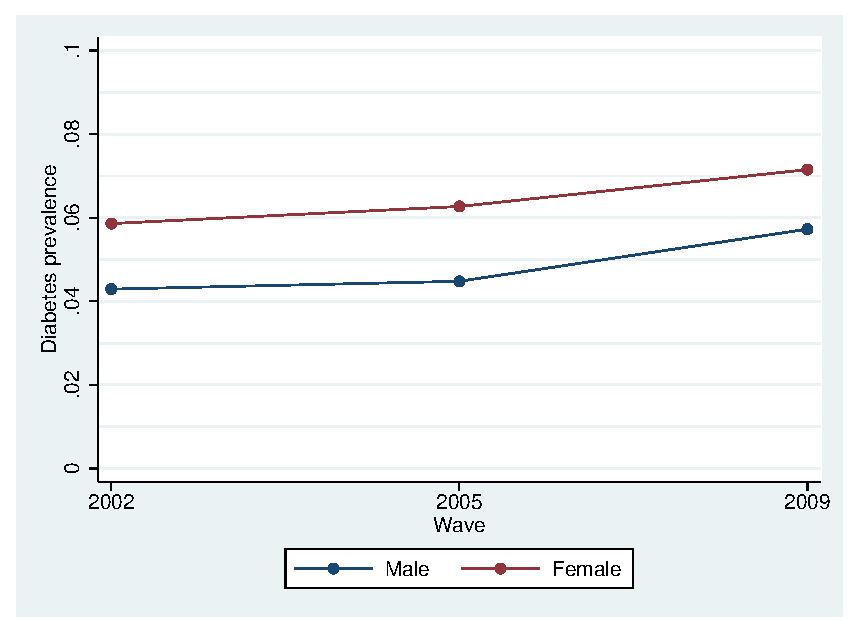
\includegraphics[width=0.7\columnwidth]{figures/diabetes_prevalence1/diabetes_prevalence1}
\end{center}
\caption{\label{fig:Self-reported-diabetes-prevalenc}Self-reported diabetes
prevalence in MxFLS}
\end{figure}

For the pooled data of all three waves (Table  \ref{tab:Pooled-sample-characteristics}),
diabetes was self-reported by 5 percent of men and 6.2 percent of
women. Most of the respondents in the sample either live in rural
or in large urbanized areas. Looking at our outcome variables, 86
percent of men report some form of employment compared to 36 percent
of women. Interestingly, men do not report higher hourly wages compared
to women but work more hours per week. Also, men are working more
often in agricultural jobs while women are more likely to be self-employed
or in non-agricultural employment. Women also have lower educational
\DIFdelbegin \DIFdel{attainments }\DIFdelend \DIFaddbegin \DIFadd{attainment }\DIFaddend on average. 
\DIFdelbegin \DIFdel{Looking at diabetes, women have a higher self-reported
diabetes prevalence. 
}\DIFdelend 

\begin{table}[h]
\caption{\label{tab:Pooled-sample-characteristics}Pooled sample characteristics (2002, 2005-2006, \DIFdelbeginFL \DIFdelFL{2009-2011}\DIFdelendFL \DIFaddbeginFL \DIFaddFL{2009-2012}\DIFaddendFL )}
\begin{center}
%\resizebox{\textwidth}{!}{%
\begin{adjustbox}{max width=\textwidth}

{ \def\sym#1{\ifmmode^{#1}\else\(^{#1}\)\fi} \begin{tabular}{l*{2}{cccc}}
\toprule
                    &\multicolumn{4}{c}{Males}                          &\multicolumn{4}{c}{Females}                        \\
                    &        Mean&          SD&         Min&         Max&        Mean&          SD&         Min&         Max\\
\midrule
\textbf{Dependent variables} &&&&&&&& \\
Employed            &       0.861&       0.346&       0.000&       1.000&       0.359&       0.480&       0.000&       1.000\\
Hourly wage             &      42.165&     483.712&       1.010&   55384.590&      41.260&     168.405&       1.007&    8803.946\\
Log hourly wage     &       3.165&       0.882&       0.010&      10.922&       3.143&       0.956&       0.007&       9.083\\
Usual weekly working hours&      46.819&      16.758&       4.000&     112.000&      38.957&      18.908&       4.000&     112.000\\
Agricultural worker &       0.222&       0.416&       0.000&       1.000&       0.043&       0.202&       0.000&       1.000\\
Self-employed       &       0.189&       0.392&       0.000&       1.000&       0.277&       0.448&       0.000&       1.000\\
Non-agricultural worker or employee&       0.589&       0.492&       0.000&       1.000&       0.680&       0.467&       0.000&       1.000\\
\textbf{Diabetes variables} &&&&&&&& \\
Diagnosed diabetes  &       0.050&       0.219&       0.000&       1.000&       0.063&       0.243&       0.000&       1.000\\
Diabetes duration   &       0.359&       2.044&       0.000&      38.000&       0.416&       2.362&       0.000&      65.000\\
\textbf{Other selected control variables} &&&&&&&& \\
\hspace*{10mm}\emph{Demographics}&&&&&&&& \\
Age of respondent   &      37.151&      13.382&      15.000&      64.000&      37.036&      13.063&      15.000&      64.000\\
Living in rural area&       0.441&       0.497&       0.000&       1.000&       0.433&       0.495&       0.000&       1.000\\
Married             &       0.549&       0.498&       0.000&       1.000&       0.536&       0.499&       0.000&       1.000\\
Number of children (<6) in household&       1.482&       1.446&       0.000&      11.000&       1.577&       1.478&       0.000&      13.000\\
Indigenous group    &       0.189&       0.391&       0.000&       1.000&       0.183&       0.387&       0.000&       1.000\\
\hspace*{10mm}\emph{Education}&&&&&&&& \\
Secondary           &       0.302&       0.459&       0.000&       1.000&       0.300&       0.458&       0.000&       1.000\\
High school         &       0.154&       0.361&       0.000&       1.000&       0.132&       0.338&       0.000&       1.000\\
Higher education    &       0.113&       0.317&       0.000&       1.000&       0.091&       0.287&       0.000&       1.000\\
\midrule
Observations        &       21739&            &            &            &       28174&            &            &            \\
\bottomrule
\end{tabular}%
}
\end{adjustbox}
\end{center}
\DIFdelbeginFL %DIFDELCMD < 

%DIFDELCMD < %%%
\DIFdelendFL \end{table}

\DIFdelbegin \DIFdel{When looking at }\DIFdelend \DIFaddbegin \DIFadd{Table \ref{tab:Biomarker-sample-characteristics} presents }\DIFaddend the descriptive statistics from the subsample of the third wave (2009-2012)\DIFaddbegin \DIFadd{, which is the one }\DIFaddend containing biomarker data\DIFdelbegin \DIFdel{in Table \ref{tab:Biomarker-sample-characteristics}, it first has to be noted }\DIFdelend \DIFaddbegin \DIFadd{. It is important to note }\DIFaddend that in this subsample respondents are somewhat older on average than in the pooled sample, which can be explained by the fact that everybody above the age of 44 was included \DIFdelbegin \DIFdel{and }\DIFdelend \DIFaddbegin \DIFadd{in the biomarker measurement, together with }\DIFaddend only a random subsample of those \DIFdelbegin \DIFdel{younger }\DIFdelend \DIFaddbegin \DIFadd{aged 44 or below }\DIFaddend \cite{Crimmins2015}. Also, self-reported diabetes is \DIFdelbegin \DIFdel{much }\DIFdelend \DIFaddbegin \DIFadd{considerably }\DIFaddend higher than in the pooled sample as well as in the full sample of wave 3. Regarding the other control and outcome variables, the sample is \DIFdelbegin \DIFdel{pretty }\DIFdelend \DIFaddbegin \DIFadd{fairly }\DIFaddend similar to the pooled sample. The added value of this subsample is obviously the biomarker information regarding diabetes. Apparently a large share of the subsample has an \ac{HbA1c} indicative of diabetes.\footnote{In one of the first analyzes of these new biomarker data \citet{Frankenberg2015} show that the rates in Mexico of elevated \DIFdelbegin \DIFdel{ac}%DIFDELCMD < {%%%
\DIFdel{HbA1c}%DIFDELCMD < } %%%
\DIFdelend \DIFaddbegin \ac{HbA1c} \DIFaddend levels are very high when compared to \ac{HbA1c} data from similar surveys in the \ac{USA} and China\DIFdelbegin \DIFdel{and note }\DIFdelend \DIFaddbegin \DIFadd{. This study also notes }\DIFaddend that "The extremely high levels of elevated \DIFdelbegin \DIFdel{HbA1c }\DIFdelend \DIFaddbegin \ac{HbA1c} \DIFaddend among Mexicans adults (...) is profoundly troubling." \DIFaddbegin \DIFadd{\mbox{%DIFAUXCMD
\citep[p.18]{Frankenberg2015}
}%DIFAUXCMD
}\DIFaddend .} In \DIFdelbegin \DIFdel{the sample used in this study }\DIFdelend \DIFaddbegin \DIFadd{our Mexican sample }\DIFaddend over 18 percent of males and females \DIFdelbegin \DIFdel{are undiagnosed }\DIFdelend \DIFaddbegin \DIFadd{result as having undiagnosed diabetes}\DIFaddend . These first descriptive results suggest that using self-reported diabetes as a measure for diabetes in Mexico can lead to a strong underestimate of the true diabetes population which potentially has consequences for the interpretation of empirical results of economic studies using self-reported diabetes data. In the \DIFdelbegin \DIFdel{ensuing }\DIFdelend \DIFaddbegin \DIFadd{following }\DIFaddend sections we will therefore try to shed some light on how taking the large undiagnosed population into account could affect the \DIFaddbegin \DIFadd{impact }\DIFaddend estimates of diabetes \DIFdelbegin \DIFdel{in relation to }\DIFdelend \DIFaddbegin \DIFadd{on }\DIFaddend labor outcomes. 

\begin{table}[h!]
\caption{\label{tab:Biomarker-sample-characteristics}Biomarker sample characteristics(2009-2012)}
\begin{center}
\begin{adjustbox}{max width=\textwidth}
{ \def\sym#1{\ifmmode^{#1}\else\(^{#1}\)\fi} \begin{tabular}{l*{2}{cccc}}
\toprule
                    &\multicolumn{4}{c}{Males}                          &\multicolumn{4}{c}{Females}                        \\
                    &        Mean&          SD&         Min&         Max&        Mean&          SD&         Min&         Max\\
\midrule
\textbf{Dependent variables} &&&&&&&& \\
Employed            &       0.860&       0.347&       0.000&       1.000&       0.339&       0.474&       0.000&       1.000\\
Hourly wage            &      36.271&      53.612&       1.128&    1038.462&      35.470&      44.000&       1.274&     461.538\\
Log hourly wage     &       3.166&       0.859&       0.121&       6.945&       3.143&       0.915&       0.242&       6.135\\
Usual weekly working hours&      46.011&      16.860&       4.000&     112.000&      38.136&      19.673&       4.000&      97.000\\
Agricultural worker &       0.252&       0.434&       0.000&       1.000&       0.035&       0.185&       0.000&       1.000\\
Self-employed       &       0.213&       0.410&       0.000&       1.000&       0.321&       0.467&       0.000&       1.000\\
Non-agricultural worker or employee&       0.535&       0.499&       0.000&       1.000&       0.644&       0.479&       0.000&       1.000\\
\textbf{Diabetes variables} &&&&&&&& \\
Glycated hemoglobin (HbA1c)&       6.459&       1.888&       4.000&      14.000&       6.565&       2.020&       4.000&      14.000\\
HbA1c $\geq 6.5\%$&       0.262&       0.440&       0.000&       1.000&       0.273&       0.446&       0.000&       1.000\\
Undiagnosed diabetes&       0.184&       0.387&       0.000&       1.000&       0.182&       0.386&       0.000&       1.000\\
Diagnosed diabetes  &       0.094&       0.291&       0.000&       1.000&       0.115&       0.319&       0.000&       1.000\\
Diabetes duration   &       0.689&       2.850&       0.000&      38.000&       0.863&       3.395&       0.000&      40.000\\
\textbf{Other selected control variables} &&&&&&&& \\
\hspace*{10mm}\emph{Demographics}&&&&&&&& \\
Age of respondent   &      42.749&      14.287&      15.000&      64.000&      42.405&      14.084&      15.000&      64.000\\
Rural village of <2,500&       0.505&       0.500&       0.000&       1.000&       0.463&       0.499&       0.000&       1.000\\
Married             &       0.603&       0.489&       0.000&       1.000&       0.559&       0.497&       0.000&       1.000\\
Number of children (<6) in household&       1.185&       1.288&       0.000&       8.000&       1.229&       1.320&       0.000&      11.000\\
Indigenous group    &       0.188&       0.391&       0.000&       1.000&       0.180&       0.384&       0.000&       1.000\\
\hspace*{10mm}\emph{Education}&&&&&&&& \\
Secondary           &       0.264&       0.441&       0.000&       1.000&       0.262&       0.440&       0.000&       1.000\\
High school         &       0.138&       0.344&       0.000&       1.000&       0.123&       0.329&       0.000&       1.000\\
Higher education    &       0.117&       0.322&       0.000&       1.000&       0.088&       0.283&       0.000&       1.000\\
\midrule
Observations        &        2792&            &            &            &        3695&            &            &            \\
\bottomrule
\end{tabular}%
}
\end{adjustbox}
\end{center}
\end{table}  



\section{\label{sec:Estimation Strategy}Estimation \DIFdelbegin \DIFdel{Strategy}\DIFdelend \DIFaddbegin \DIFadd{strategy}\DIFaddend }

  
The conceptual framework of our study is based on the work of \citet{Strauss1998},   who specify the following model \DIFdelbegin \DIFdel{to }\DIFdelend of the relationship \DIFdelbegin \DIFdel{of }\DIFdelend \DIFaddbegin \DIFadd{between }\DIFaddend health and labor market outcomes, i.e. labor force participation and labor supply conditional on health and wages.
\begin{equation}
L=L(H, pc, w(H;S,A,B,I,\alpha,e_{w}), S, A, B, V, \xi) \label{eq:wage}
\end{equation}
where $L$ is labor supply or labor market participation, $pc$ is a vector of prices for consumer goods, $w$ is the real wage; $H$ is an array of measured health human capital; $S$ is education; $A$ is a vector of demographic characteristics; $B$ is the family background of the individual; $I$ is local community infrastructure; $\alpha$ is an array of unobservables such as ability and $e_w$ is measurement error, $V$ is non-labor income and $\xi$ is the taste parameter. 

The equation showcases the joint effect of health on both wages and labor supply or labor market participation. Health affects labor supply and participation indirectly by changing wages and directly by impacting the ability to work.

There are several ways diabetes may affect $H$. First of all, diabetes can deteriorate health if it remains untreated with the adverse effects increasing over time. Second, a diagnosis of diabetes and ensuing treatment may lead to better health compared to the undiagnosed state\DIFdelbegin \DIFdel{, however}\DIFdelend \DIFaddbegin \DIFadd{. However}\DIFaddend , compared to healthy people even those with diabetes receiving treatment may still have worse health outcomes. Third, there is also evidence that the diagnosis itself may affect one's own health perception and can lead to worse self-perceived health \citep{Thoolen2006a}. We therefore expect diabetes to adversely affect health and consequently labor market outcomes.

When estimating equation  \ref{eq:wage} empirically with observational data, unobserved heterogeneity may bias the results. As mentioned in section  \ref{sec:Introduction} unobserved factors captured in $\alpha$ such as early childhood investments, innate ability and time preference could affect wages as well as the probability to develop diabetes. Further, changes in lifestyle due to changes in wages or employment status may also affect the probability to develop diabetes \DIFdelbegin \DIFdel{though }\DIFdelend \DIFaddbegin \DIFadd{through }\DIFaddend changes in diet and physical activity patterns. Finally, measurement error $e_w$ may be an important issue due to the large undiagnosed population with diabetes, particularly if being diagnosed is related to employment or wages via better access to healthcare through employment benefits and higher income.

In the following section we \DIFdelbegin \DIFdel{will show how we will }\DIFdelend \DIFaddbegin \DIFadd{describe how we }\DIFaddend deal with these issues in our estimation strategy.


\subsection{Panel data estimation strategy: Self-reported Diabetes}

We investigate the relationship of self-reported diabetes and three
labor market outcomes, i.e. employment chances, log hourly wages
and normal weekly working hours using a fixed effects model. While using individual level \ac{FE} does not fully
identify a causal relationship, as other forms of heterogeneity could
affect our estimates (i.e. via time-variant unobserved heterogeneity
or simultaneity) it does improve on the degree of causal inference,
compared to a simple cross-sectional analysis\DIFdelbegin \DIFdel{, and in }\DIFdelend \DIFaddbegin \DIFadd{. In }\DIFaddend particular it
does allow to control for unobserved personal characteristics that
could bias the estimates, without the drawbacks of a less than convincing
\ac{IV} strategy that has been widely applied in this literature. 
For comparison purposes we also present the results of the respective random effects models that assume no unobserved heterogeneity.

We estimate a two-part model where the model for employment chances
takes the following form:

\noindent 
\begin{equation}
Y_{it}=\beta_{0}+\beta_{1}Diabetes_{it}+\beta_{2}X_{it}+c_{i}+\gamma_{t}+u_{it}.\label{eq:employed}
\end{equation}


where $Y_{it}$ is a binary variable taking a value of $1$ if respondent
$i$ reports being employed at time $t$ and $0$ otherwise, $Diabetes_{it}$
is a binary variable taking a value of $1$ at time $t$ if the respondent
reports having ever received a diagnosis of diabetes, $X_{it}$ is
a vector of control variables, $c_{i}$ represents an individual fixed
effect, $\gamma_{t}$ represents a year fixed effect, and $u_{it}$
is the error term.

For the relationship of self-reported diabetes with log hourly wages
and weekly working hours \DIFaddbegin \DIFadd{our empirical }\DIFaddend models are estimated conditional on having positive wages and being
employed, respectively. In these models $Y_{it}$ represents the log hourly wage
of respondent $i$ at time $t$ or the usual weekly working hours
over the last year.

The log hourly wage was calculated by adding up the reported monthly
income from the first and potential second job and dividing it by
4.33 which corresponds to the average number of weeks per month in
a year with 52 weeks. This gave us the average earnings per week which
was then divided by the usual weekly working hours to arrive at an
hourly wage estimate\footnote{\DIFdelbegin \DIFdel{labor }\DIFdelend \DIFaddbegin \DIFadd{Labor }\DIFaddend income was either reported as the total amount for the whole
month or if possible more detailed containing information on the monthly
wage, income from piecework, tips, extra hours, meals, housing, transport,
medical benefits and other earnings. Over 80 percent of respondents
reported the total amount instead of a detailed amount. Respondents
were also asked for their yearly income and we used that information
to arrive at an hourly wage if information for monthly labor income
was missing.} Finally, we adjusted the calculated wage for inflation from the year
of the interview up to 2013. Working hours were calculated summing
up the self-reported usual working hours of the first and potential
second job. We dropped 39 observations where the sum of working hours
exceeded 112 hours per week, i.e. more than 16 hours of work per day
on each day of the week as we deemed these reports to be unrealistic.
Due to a considerable number of missing values the sample used for the wage estimation is considerably smaller than the model for working hours.

The control variables in both \ac{FE} specifications include dummy variables for the effects of any changes in the living environment
of living in a small, medium or large city with rural and state
dummies capturing the effects of moving to a different state. We also include a marital
status dummy to control for the impact of marriage on employment chances.
A variable capturing the number of children residing in the household
below the age of 18 is used to control for the impact of children
on labor market outcomes and the effect of childbearing and related
gestational diabetes on the probability of developing type 2 diabetes
\citep{Bellamy2009}. To account for the effect that changes in household
wealth might have on diabetes and employment chances, we use standard
principal component analysis of multiple indicators of household assets
and housing conditions to create an indicator for household wealth
\citep{Filmer2001}. The components used for the construction of the
wealth index are detailed in \citet{Seuring2015}. Finally, calender year fixed effects are included to capture the effects of increasing age and any macroeconomic shocks over time.

Additionally, we estimate models using a self-reported
measure of the years since diagnosis \DIFdelbegin \DIFdel{instead }\DIFdelend \DIFaddbegin \DIFadd{in order }\DIFaddend to explore the \DIFdelbegin \DIFdel{temporal nature of diabetes . First, using }\DIFdelend \DIFaddbegin \DIFadd{role of the duration of diabetes in affecting labor outcomes. We start by following }\DIFaddend a linear specification
indicating the association of labor market outcomes with each additional
year since diagnosis, \DIFdelbegin \DIFdel{using the following specification}\DIFdelend \DIFaddbegin \DIFadd{as follows}\DIFaddend :

\begin{equation}
Y_{it}=\beta_{0}+\beta_{1}Dyears_{it}+\beta_{2}X_{it}+c_{i}+\gamma_{t}+u_{it},\label{eq:duration_linear}
\end{equation}


\noindent where $\beta_{1}Dyears_{it}$ is a continuous variable indicating
years since first diabetes diagnosis.

\DIFdelbegin \DIFdel{Second, }\DIFdelend \DIFaddbegin \DIFadd{In an effort }\DIFaddend to capture possible non-linearities in the relationship of interest we \DIFaddbegin \DIFadd{then }\DIFaddend use a spline function that allows the effect
of an additional year with diabetes to vary over time.
\begin{equation}
Y_{it}=\delta_{0}+g(Dyears_{it})+\delta_{2}X_{it}+c_{i}+\gamma_{t}+u_{it}.\label{eq:splines}
\end{equation}


\noindent with $g(Dyears_{it})=\sum_{n=1}^{N}\delta_{n}\cdot max\{Dyears_{it}-\eta_{n-1}\}I_{in}$
and $I_{in}=1[\eta_{n-1}\leq Dyears_{it}<\eta_{n}]$, with $\eta_{n}$
being the place of the $n$-th node for $n=1,2,\ldots,N$. We choose
three nodes that - based on visual inspection (see Figures \ref{fig:Kernel-weighted-local-polynomial_empl}, \ref{fig:Kernel-weighted-local-polynomial_wage} and \ref{fig:Kernel-weighted-local-polynomial_workhrs} in the
result section) - best captured any possible non-linearity in the
relationship \DIFdelbegin \DIFdel{of }\DIFdelend \DIFaddbegin \DIFadd{between }\DIFaddend diabetes duration and \DIFdelbegin \DIFdel{our dependent variables}\DIFdelend \DIFaddbegin \DIFadd{labor outcomes}\DIFaddend . These
are located at four, eleven and twenty years after diagnosis. The
first four years should capture any immediate effects of the diagnosis,
the years five to eleven should capture any effects of adaptation to
the disease. After eleven years it is conceivable that many of the
debilitating complications of diabetes would appear that could deteriorate
health and lead to adverse effects on \DIFdelbegin \DIFdel{our }\DIFdelend labor market outcomes.
The coefficient$\delta_{n}$ captures the effect of diabetes for the
$n$-th interval. The effects are linear if $\delta_{1}=\delta_{2}=,\ldots,=\delta_{n}$.

Because the year of diagnosis was only reported in the third wave,
duration of diabetes (or time since diagnosis)
for the earlier waves was only calculated for those that had also responded to the third
wave. To arrive at the time passed since diagnosis, the year of diagnosis
was subtracted from the year of the interview. In order to have zero years representing people without a self-reported  diagnosis, those that reported
a diagnosis in the year of the interview were counted as 'one year
since diagnosis'. Accordingly, if the respondent reported to having
been diagnosed in the year before the interview he or she was counted
as 'two years since diagnosis' and so on.

\subsection{Cross-section data estimation strategy: biomarker and self-reported data}

Self-reported diabetes only captures part of the diabetes population as many individuals remain undiagnosed.  Estimations based on self-reports may therefore suffer from a selection bias.

The issue of measurement error can be depicted in a simple theoretical model. Assuming that the true model of the effect of diabetes on labor market outcomes is $y^{*}=X^{*}\beta+\epsilon$ where $y^{*}$ and $\epsilon$ are scalars and $X^{*}$ and $\beta$ are vectors. Because we do not observe the true values of $y^{*}$ and $X^{*}$  we have to use reported measures that contain errors: $X=X^{*} + u$ and $y=y^{*} + v$. In the case of diabetes as a right-hand side variable, measurement error cannot be classical as it is negatively correlated with the true diabetes status. Hence, the direction of the bias is unknown and cannot be assumed to be attenuating\DIFdelbegin \DIFdel{making inference based on self-reported measures without some information about the direction of a potential bias difficult}\DIFdelend .

Self-report of diabetes can lead to errors due to two main factors: 
\begin{enumerate}
\item \textbf{Systematic overreporting of diabetes:} people without diabetes
could intentionally report a diabetes diagnosis with a view to justifying
some other adverse event or status in their life (e.g. being unemployed). 
\item \textbf{Systematic underreporting of diabetes:} it is conceivable
that people with diabetes \DIFdelbegin \DIFdel{are ashamed of their disease }\DIFdelend \DIFaddbegin \DIFadd{feel bad about suffering from the condition }\DIFaddend and therefore
do not report it. Further, diabetes often remains
undiagnosed for long periods of time or is not diagnosed at all, potentially
leaving many people unaware of the disease which hence results in
the non-report of the disease.
\end{enumerate} 

Overreporting could attenuate the coefficient of diabetes as those falsely reporting a diabetes diagnosis experience no adverse health
effects of diabetes that could affect labor outcomes. However, if some of those misreports were
made in order to justify some other adverse event, e.g. current unemployment
or other health problems, then this could potentially lead to an overestimation
of the true effect of diabetes on employment. Underreporing due to
a non-diagnosis could cause either an overestimation or attenuation
bias: it would lead to an overestimation if people with undiagnosed
diabetes were generally healthier and therefore more likely to have
positive labor market outcomes than people with diagnosed diabetes
and would therefore have attenuated the effect of diabetes if they
were observed in the data. Yet, because they are unobserved\DIFaddbegin \DIFadd{, }\DIFaddend the effect
of diabetes using self-reports may be overstated. However, if those
with undiagnosed diabetes were very similar in terms of health to those with
diagnosed diabetes and consequently experienced similar health problems
that adversely affected their labor market outcomes, then this would lead to an attenuation of the diabetes coefficient as the control group without observed diabetes, i.e. including people with undiagnosed
diabetes, were on average less healthy and have worse labor market outcomes than it
would have had\DIFaddbegin \DIFadd{, }\DIFaddend if all diabetes cases had been observed.

In this context, however, an important additional issue arises with the potential effect that being informed via a diabetes diagnosis
might have on labor market outcomes. In assessing the labor market
effects of diabetes with the help of self-reported diabetes as our
diabetes indicator, we need to be aware that we could be \DIFdelbegin \DIFdel{measuring
something else then }\DIFdelend \DIFaddbegin \DIFadd{capturing 
something other than }\DIFaddend the pure health effects of diabetes. A diabetes
diagnosis is likely to also affect an individual's psychology and
health behaviour which in turn could have its own effects on economic
outcomes. One study found a diabetes diagnosis and subsequent treatment
to increase the odds of psychological problems, including depression
and anxiety \citep{Thoolen2006a}. Other research has also shown that
anxiety and depression increase with the number of diabetes symptoms
people with diabetes self-report after a diagnosis \cite{Paddison_2011}.
Interestingly, similar results have not been found for people with
undiagnosed diabetes \citep{Nouwen2011}. When looking at economic
studies of the effect of a diabetes diagnosis, \citet{Liu2014} found
that receiving a diabetes diagnosis considerably reduced labor income
in Chinese employees shortly after their diagnosis. Similarly, others
have shown that a hypertension diagnosis can affect health
behaviours, \DIFdelbegin \DIFdel{i.e.a reduce }\DIFdelend \DIFaddbegin \DIFadd{e.g. in the form of a reduction in }\DIFaddend fat intake \citep{Zhao2013a}. Similar effects have also been found
for the \DIFdelbegin \DIFdel{US}\DIFdelend \DIFaddbegin \DIFadd{USA}\DIFaddend , in that people receiving a diabetes diagnosis changed
their health behaviours favourably, albeit only over the short term
\citep{Slade2012}. It is not difficult to imagine that such changes in
health behaviours resulting from a diabetes diagnosis might also translate
into changes in employment chances or productivity, on top of a potential
effects resulting from the diabetes-related health changes. Hence, the labor market effects we measure with self-reported diabetes are likely different from those
that we would measure based on a purely medical assessment of diabetes
obtained from blood tests, not only due to measurement error but also
due to the additional information effects of the diagnosis itself.

We use the biomarker data in wave three to explore the relationship of measured diabetes, including undiagnosed diabetes with labor outcomes and compare it to estimates using self-reported diabetes. The biomarker data also allows us to look at diabetes severity, as measured
by \ac{HbA1c} values. Since this data is only available for one wave - the
last wave \DIFdelbegin \DIFdel{, }\DIFdelend \DIFaddbegin \DIFadd{- }\DIFaddend we focus on a cross-section analysis. Moreover,
as mentioned above, biomarkers were only taken from about one-third  of the initial representative sample, which leaves
us with information on 6994 survey participants. Therefore the analysis
cannot be directly compared to the panel-based results in this paper.
Nonetheless, it allows for a first exploration of the relationships
of undiagnosed diabetes as well as disease severity with labor market
outcomes.  It further allows us to explore
some of the heterogeneity that may exist within the diabetes population
in terms of how well different people manage their diabetes condition.
We first estimate a model to investigate the association of objectively
measured diabetes (HbA1c $\geq6.5\%$) with labor market outcomes
taking the following form: 
\begin{equation}
Y_{i}=\beta_{0}+\beta_{1}Dobj_{i}+\beta_{2}X_{i}+u_{i}\label{eq:diab_objective}
\end{equation}
where $\beta_{1}Dobj_{i}$ is equal to $1$ if HbA1c $\geq6.5\%$.
In a further step we estimate the following equation 
\begin{equation}
Y_{i}=\beta_{0}+\beta_{1}Dsr_{i}+\beta_{1}Dud_{i}+\beta_{2}X_{i}+u_{i}.\label{eq:diab_sr_ud}
\end{equation}
to investigate how the associations differ between people with diagnosed
and undiagnosed diabetes. $\beta_{1}Dsr_{i}$ identifies those diagnosed
and is equal to $1$ if the person self-reported a diabetes diagnosis.
$\beta_{1}Dud_{i}$ identifies those undiagnosed and is equal to $1$
if the person did not self-report a diabetes diagnosis but has an
HbA1c $\geq6.5\%$.




Before moving on to the results \DIFdelbegin \DIFdel{we want to stress, }\DIFdelend \DIFaddbegin \DIFadd{it bears emphasising }\DIFaddend that despite our efforts to reduce any bias in our estimates we do not make any causal claims as the used methods cannot prove causation. While the fixed effects model accounts for time invariant
unobserved confounders, it is still possible that the estimates are biased
due to important time variant heterogeneity we did not account for, or
due to labor market outcomes simultaneously affecting the chances to develop or
being diagnosed with diabetes. For example\DIFaddbegin \DIFadd{, }\DIFaddend changes in lifestyle due to
employment or unemployment could affect the probabilities of developing
diabetes which then in turn could affect labor market outcomes. Another pathway could be high stress levels at
work that have been shown to have a positive association with
diabetes incidence for obese women and a negative association for
non-obese men \citep{Heraclides2012,Eriksson2013}. However, part
of the possible effects of work stress on diabetes should be accounted
for by our fixed effects model. Genetics play an important role for
the development of type 2 diabetes and it is likely that people with
a genetic predisposition are more likely to develop diabetes due
to stress. Further, coping mechanism related to stress are also likely
to differ between persons depending on their genetics and coping
methods learned early in life \citep{Schneiderman2005}, so that our
fixed effect technique should account for these time invariant factors\DIFdelbegin \DIFdel{and reduce }\DIFdelend \DIFaddbegin \DIFadd{, 
reducing }\DIFaddend the possible bias. Also the literature on the effects of employment
status on diabetes so far has not found strong adverse effects of being laid
off on diabetes self-reports \citep{Bergemann2011,Schaller2015},
\DIFdelbegin \DIFdel{albeit only for }\DIFdelend \DIFaddbegin \DIFadd{although this has only been researchers in a }\DIFaddend high-income \DIFdelbegin \DIFdel{countries}\DIFdelend \DIFaddbegin \DIFadd{country context so far}\DIFaddend .

\section{\label{sec:RESULTS} Results}


\subsection{Panel data analysis}

\subsubsection*{Self-reported diabetes}

Table \ref{tab:Self-reported-diabetes-and} presents the estimation
results of the \ac{FE} model \ref{eq:employed}.
The results indicate significant and substantial reductions in employment
chances for people with self-reported diabetes. The effects are surprisingly similar between males and females showing a reduction in
employment chances of around 6.5 percentage points. The adverse effects on employment confirm findings of an earlier study on Mexico by \cite{Seuring2015} albeit \DIFdelbegin \DIFdel{we now find a }\DIFdelend \DIFaddbegin \DIFadd{with a now }\DIFaddend stronger indication of an effect for females. This earlier study used an \ac{IV} approach and found diabetes to be exogenous in the determination of employment chances, a finding which is supported by the small difference between our \ac{RE} and \ac{FE} estimates for employment chances.
\begin{table}[h]
\caption{\label{tab:Self-reported-diabetes-and}Self-reported diabetes and labor market outcomes }
\begin{center}
%\resizebox{\textwidth}{!}{%
\begin{adjustbox}{max width=\textwidth}
{
\def\sym#1{\ifmmode^{#1}\else\(^{#1}\)\fi} \begin{tabular}{l*{9}{SS}}
\toprule
                &\multicolumn{3}{c}{Employment}                          &\multicolumn{3}{c}{Log hourly wages}                    &\multicolumn{3}{c}{Weekly working hours}                  \\\cmidrule(lr){2-4}\cmidrule(lr){5-7}\cmidrule(lr){8-10}
                &\multicolumn{1}{c}{(1)}&\multicolumn{1}{c}{(2)}&\multicolumn{1}{c}{(3)}&\multicolumn{1}{c}{(4)}&\multicolumn{1}{c}{(5)}&\multicolumn{1}{c}{(6)}&\multicolumn{1}{c}{(7)}&\multicolumn{1}{c}{(8)}&\multicolumn{1}{c}{(9)}\\
                &\multicolumn{1}{c}{Pooled}&\multicolumn{1}{c}{Males}&\multicolumn{1}{c}{Females}&\multicolumn{1}{c}{Pooled}&\multicolumn{1}{c}{Males}&\multicolumn{1}{c}{Females}&\multicolumn{1}{c}{Pooled}&\multicolumn{1}{c}{Males}&\multicolumn{1}{c}{Females}\\
\midrule
\multicolumn{10}{l}{\textit{Fixed Effects}}\\
Diagnosed diabetes&    -.066\sym{***}&    -.065\sym{**} &    -.065\sym{***}&     .033         &     .009         &     .100         &    -.853         &    -.225         &   -2.346         \\
                &   (.018)         &   (.025)         &   (.024)         &   (.064)         &   (.066)         &   (.158)         &  (1.269)         &  (1.458)         &  (2.518)         \\
\midrule
\multicolumn{10}{l}{\textit{Random Effects}}\\
Diagnosed diabetes&    -.068\sym{***}&    -.071\sym{***}&    -.057\sym{***}&     .067\sym{**} &     .110\sym{***}&    -.017         &    -.841         &    -.575         &   -1.742         \\
                &   (.009)         &   (.013)         &   (.012)         &   (.031)         &   (.037)         &   (.058)         &   (.604)         &   (.704)         &  (1.134)         \\
N               &    49323         &    21801         &    27522         &    20974         &    13925         &     7049         &    26882         &    17801         &     9081         \\
\bottomrule
\multicolumn{10}{l}{\footnotesize Robust standard errors in parentheses}\\
\multicolumn{10}{l}{\footnotesize Other control variables: state dummies, urbanization dummies, education dummies, married dummy, number children < 6}\\
\multicolumn{10}{l}{\footnotesize wealth, age and calender year fixed effects}\\
\multicolumn{10}{l}{\footnotesize The random effects model additionally controls for initial age when entering the survey, being indigenous and gender}\\
\multicolumn{10}{l}{\footnotesize The wage and working hour models additionally control for type of work (agricultural and self employed with}\\
\multicolumn{10}{l}{\footnotesize non-agricultural employment as the base) and for health insurance status}\\
\multicolumn{10}{l}{\footnotesize \sym{*} \(p<0.10\), \sym{**} \(p<0.05\), \sym{***} \(p<0.01\).}\\
\end{tabular}%
}
%}
\end{adjustbox}
\end{center}
\end{table}

While the adverse relationship between self-reported diabetes and
employment chances appears to be quite strong, we find no evidence
for any relationship with wages or working hours using the \ac{FE} specification. Further, comparing the results with the \ac{RE} model, we see that there are no stark differences for employment chances but that the \ac{FE} model appears to correct for a positive bias in the effect of diabetes on wages. The \ac{RE} model suggests \DIFaddbegin \DIFadd{-- counter-intuitively -- }\DIFaddend that men with diabetes earn more than men without diabetes\DIFdelbegin \DIFdel{which is an unintuitive finding}\DIFdelend . Controlling for fixed unobservables, however, the positive effect disappears and becomes insignificant suggesting that assuming exogeneity of diabetes leads to biased estimates of wages. A potential explanation is that men with a comparatively higher innate ability are able to earn higher wages and at the same time to better manage their diabetes preventing them from dropping out of the labor market due to health reasons. They may also be more valuable to their employers preventing them from being dismissed even if the employer would normally discriminate against people with diabetes.

To investigate whether there are differences in
wages and working hours between different types of work, we estimate
a model including interaction terms between self-reported diabetes
and agricultural employment and between self-reported diabetes and
self-employment, respectively, using non-agricultural employment as
the \DIFdelbegin \DIFdel{base}\DIFdelend \DIFaddbegin \DIFadd{benchmark}\DIFaddend . There would be reason to expect the relationship between
diabetes and labor market outcomes to differ with the type of work\DIFaddbegin \DIFadd{, }\DIFaddend as
the health consequences of diabetes could affect the productivity
of workers by reducing their physical abilities. Accordingly, people
with diabetes working in an agricultural job that requires strenuous,
physical efforts to work the land could see their productivity \DIFdelbegin \DIFdel{to be
}\DIFdelend \DIFaddbegin \DIFadd{being
}\DIFaddend more adversely affected by diabetes than those working in an office,
hence being less physically active. 

\DIFdelbegin %DIFDELCMD < \begin{table}[h]
%DIFDELCMD < %%%
\DIFdelend \DIFaddbegin \begin{table}[!ht]
\DIFaddendFL \caption{\label{tab:Self-reported-diabetes-interaction}Relationship of self-reported diabetes by type of work and wages and working hours}
\begin{center}
%\resizebox{\textwidth}{!}{%
\begin{adjustbox}{max width=\textwidth}
{
\def\sym#1{\ifmmode^{#1}\else\(^{#1}\)\fi}
\begin{tabular}{l*{6}{SS}}
\toprule
                &\multicolumn{3}{c}{Log monthly wages (FE)}              &\multicolumn{3}{c}{Monthly work hours (FE)}             \\\cmidrule(lr){2-4}\cmidrule(lr){5-7}
                &\multicolumn{1}{c}{(1)}&\multicolumn{1}{c}{(2)}&\multicolumn{1}{c}{(3)}&\multicolumn{1}{c}{(4)}&\multicolumn{1}{c}{(5)}&\multicolumn{1}{c}{(6)}\\
                &\multicolumn{1}{c}{Pooled}&\multicolumn{1}{c}{Males}&\multicolumn{1}{c}{Females}&\multicolumn{1}{c}{Pooled}&\multicolumn{1}{c}{Males}&\multicolumn{1}{c}{Females}\\
\midrule
\multicolumn{7}{l}{\textit{Fixed Effects}}\\
Reference category: No diabetes and non-agricultural employee&&&&&& \\ \DIFdelbeginFL %DIFDELCMD < &   %%%
\DIFdelFL{(.043)         }%DIFDELCMD < &   %%%
\DIFdelFL{(.044)         }%DIFDELCMD < &   %%%
\DIFdelFL{(.190)         }%DIFDELCMD < &   %%%
\DIFdelFL{(.764)         }%DIFDELCMD < &   %%%
\DIFdelFL{(.802)         }%DIFDELCMD < &  %%%
\DIFdelFL{(2.713)         }\DIFdelendFL \\
No diabetes and agricultural worker&    -.111\sym{***}&    -.092\sym{**} &    -.294         &   -3.934\sym{***}&   -3.697\sym{***}&   -4.176         \\
                &   (.043)         &   (.044)         &   (.190)         &   (.764)         &   (.802)         &  (2.713)         \\

No diabetes and self-employed   &    -.029         &     .015         &    -.149\sym{*}  &   -2.503\sym{***}&   -1.817\sym{**} &   -4.318\sym{***}\\
                &   (.041)         &   (.045)         &   (.087)         &   (.643)         &   (.706)         &  (1.419)         \\

Diagnosed diabetes and non-agricultural employee&     .065         &     .060         &     .089         &    -.006         &     .486         &   -1.077         \\
                &   (.071)         &   (.074)         &   (.169)         &  (1.315)         &  (1.585)         &  (2.262)         \\

Diagnosed diabetes and agricultural worker&    -.209         &    -.200         &    -.394         &   -5.251\sym{*}  &   -4.950\sym{*}  &   -5.911         \\
                &   (.191)         &   (.198)         &   (.373)         &  (2.797)         &  (2.879)         & (15.395)         \\

Diagnosed diabetes and self-employed&    -.036         &    -.099         &     .128         &    -.371         &    1.078         &   -3.963         \\
                &   (.161)         &   (.188)         &   (.322)         &  (2.227)         &  (2.484)         &  (4.740)         \\
\midrule
R2 within       &     .022         &     .022         &     .031         &     .010         &     .012         &     .018         \\
\midrule
\multicolumn{7}{l}{\textit{Random Effects}}\\
Reference category: No diabetes and non-agricultural employee&&&&&& \\\DIFaddbeginFL \\
\DIFaddendFL No diabetes and agricultural worker&    -.226\sym{***}&    -.236\sym{***}&    -.220\sym{***}&   -3.536\sym{***}&   -3.429\sym{***}&   -2.512\sym{**} \\
                &   (.020)         &   (.021)         &   (.063)         &   (.352)         &   (.377)         &  (1.002)         \\

No diabetes and self-employed   &    -.038\sym{*}  &     .039         &    -.154\sym{***}&   -2.911\sym{***}&   -1.187\sym{***}&   -4.577\sym{***}\\
                &   (.022)         &   (.026)         &   (.039)         &   (.344)         &   (.408)         &   (.608)         \\

Diagnosed diabetes and non-agricultural employee&     .090\sym{***}&     .134\sym{***}&     .029         &   -1.049         &     .040         &   -3.246\sym{***}\\
                &   (.034)         &   (.041)         &   (.063)         &   (.710)         &   (.875)         &  (1.218)         \\

Diagnosed diabetes and agricultural worker&    -.132         &    -.178         &     .386         &   -2.941\sym{*}  &   -4.287\sym{***}&    1.749         \\
                &   (.112)         &   (.116)         &   (.514)         &  (1.588)         &  (1.660)         &  (5.955)         \\

Diagnosed diabetes and self-employed&    -.119         &    -.043         &    -.204         &    1.397         &     .009         &    3.391         \\
                &   (.081)         &   (.100)         &   (.133)         &  (1.324)         &  (1.596)         &  (2.290)         \\
\midrule
R2              &     .213         &     .201         &     .246         &     .067         &     .026         &     .049         \\
N               &    20974         &    13925         &     7049         &    26882         &    17801         &     9081         \\
\bottomrule
\multicolumn{7}{l}{\footnotesize Robust standard errors in parentheses}\\
\multicolumn{7}{l}{\footnotesize Other control variables: state dummies, urbanization dummies, education dummies, married dummy, number children < 6, wealth, health insurance status, age and calender year fixed effects}\\
\multicolumn{7}{l}{\footnotesize The random effects model additionally controls for initial age when entering the survey, being indigenous and gender}\\
\multicolumn{7}{l}{\footnotesize \sym{*} \(p<0.10\), \sym{**} \(p<0.05\), \sym{***} \(p<0.01\)}\\
\end{tabular}
}
%}
\end{adjustbox}
\end{center}
\end{table}  

\FloatBarrier

As Table \ref{tab:Self-reported-diabetes-interaction} shows, male
agricultural workers have lower wages generally, but the relationship
with diabetes remains unaffected by the type of work. The only
statistically more relevant relationship that we find relates to working
hours of agricultural workers with diabetes, who appear to work about
\DIFdelbegin \DIFdel{6 }\DIFdelend \DIFaddbegin \DIFadd{five }\DIFaddend hours less than non-agricultural workers without self-reported diabetes.
However, because we have more than two work types we cannot draw conclusions
solely on the basis of the t-statistic. We therefore perform a Wald
test for the overall significance of the interaction term which does
not reject the null of no interaction effects, suggesting that the
effect of diabetes on working hours does not vary significantly by type of work.
When stratified by gender, standard errors become larger, which should
be explained by the small number of observations of females with diabetes
reporting working hours in agricultural employment (n=10) compared
to men (n=139). Overall, we find no evidence for an association of
self-reported diabetes and wages or working hours.

Finally, we explore if diabetes affects the selection into employment according to the different types of work. We refrain from using a fixed effects multinomial logit model due to the problems surrounding the calculation of interpretable marginal effects \citep{Pforr2014}. We instead estimate fixed effects models of the probability of being in non-agricultural employment, agricultural employment or self-employment using three dummy variables indicating the respective type of work as the dependent variable.\footnote{For example, "non-agricultural employment" is coded as $1$ if the respondent is engaged in agricultural work and is coded as $0$ for those unemployed, in non-agricultural employment or self-employed. This is repeated for the dummy variables "agricultural employment" and "self-employed".} The results in table \ref{tab:Self-reported-diabetes-selection_LPM} indicate that for men diabetes mainly appears to be associated with reduced employment chances for those self-employed\DIFdelbegin \DIFdel{and }\DIFdelend \DIFaddbegin \DIFadd{, while }\DIFaddend for women an adverse association is found for those in agricultural and self-employment. This could suggest that having diabetes drives people out of self-employment and agricultural jobs, potentially because these jobs are more physically demanding than other forms of work and likely also because they provide less protection in terms of insurance and formal employment. We interpret the fact that the coefficient signs are negative for all types of work as an indication that people with diabetes predominantly become unemployed rather than \DIFdelbegin \DIFdel{to sort }\DIFdelend \DIFaddbegin \DIFadd{sorting }\DIFaddend into other types of work that would be better suited for them given their health \DIFaddbegin \DIFadd{status}\DIFaddend [DOES THIS INTERPRETATION MAKE SENSE?].


\begin{table}[h]
\caption{\label{tab:Self-reported-diabetes-selection_LPM}Relationship of self-reported diabetes with selection into types of work }
\begin{center}
%\resizebox{\textwidth}{!}{%
\begin{adjustbox}{max width=\textwidth}
{
\def\sym#1{\ifmmode^{#1}\else\(^{#1}\)\fi}
\begin{tabular}{l*{9}{S
S}}
\toprule
                      &\multicolumn{3}{c}{Pooled}                              &\multicolumn{3}{c}{Males}                               &\multicolumn{3}{c}{Females}                             \\\cmidrule(lr){2-4}\cmidrule(lr){5-7}\cmidrule(lr){8-10}
                &\multicolumn{1}{c}{(1)}&\multicolumn{1}{c}{(2)}&\multicolumn{1}{c}{(3)}&\multicolumn{1}{c}{(4)}&\multicolumn{1}{c}{(5)}&\multicolumn{1}{c}{(6)}&\multicolumn{1}{c}{(7)}&\multicolumn{1}{c}{(8)}&\multicolumn{1}{c}{(9)}\\
                &\multicolumn{1}{c}{Non-agric.}&\multicolumn{1}{c}{Agric.}&\multicolumn{1}{c}{Self-employed}&\multicolumn{1}{c}{Non-agric.}&\multicolumn{1}{c}{Agric.}&\multicolumn{1}{c}{Self-employed}&\multicolumn{1}{c}{Non-agric.}&\multicolumn{1}{c}{Agric.}&\multicolumn{1}{c}{Self-employed}\\
\midrule
\midrule
\multicolumn{10}{l}{ \textit{Fixed Effects}}\\
Diagnosed diabetes=1&    -.015         &    -.017\sym{*}  &    -.039\sym{***}&    -.021         &    -.009         &    -.050\sym{*}  &    -.009         &    -.022\sym{***}&    -.033\sym{*}  \\
                &   (.016)         &   (.010)         &   (.015)         &   (.029)         &   (.021)         &   (.026)         &   (.018)         &   (.009)         &   (.018)         \\
\multicolumn{10}{l}{\textit{ Random Effects}}\\
Diagnosed diabetes=1&    -.043\sym{***}&    -.044\sym{***}&     .003         &    -.053\sym{***}&    -.066\sym{***}&     .033\sym{**} &    -.042\sym{***}&    -.012\sym{***}&    -.016\sym{*}  \\
                &   (.009)         &   (.005)         &   (.008)         &   (.017)         &   (.011)         &   (.015)         &   (.010)         &   (.002)         &   (.009)         \\
\midrule
N               &    47330         &    47330         &    47330         &    20730         &    20730         &    20730         &    26600         &    26600         &    26600         \\
\bottomrule
\multicolumn{10}{l}{\footnotesize Robust standard errors in parentheses}\\
\multicolumn{10}{l}{\footnotesize Other control variables: state dummies, urbanization dummies, education dummies, married dummy, number children < 6, wealth, age and calender year fixed effects}\\
\multicolumn{10}{l}{\footnotesize The random effects model additionally controls for initial age when entering the survey, being indigenous and gender}\\
\multicolumn{10}{l}{\footnotesize \sym{*} \(p<0.10\), \sym{**} \(p<0.05\), \sym{***} \(p<0.01\)}\\
\end{tabular}
}
%}
\end{adjustbox}
\end{center}
\end{table}  

\FloatBarrier

\subsubsection*{Self-reported diabetes duration}

Because diabetes is a chronic and generally life-long disease, we investigate how soon after the first diagnosis diabetes may affect labor market outcomes. Given that complications of diabetes develop over time it could be that the effect increases
linearly as the years go by. \DIFdelbegin \DIFdel{However}\DIFdelend \DIFaddbegin \DIFadd{On the other hand}\DIFaddend , non-linear relationships
are also \DIFdelbegin \DIFdel{imaginable }\DIFdelend \DIFaddbegin \DIFadd{plausible }\DIFaddend as psychological effects of the immediate diagnosis
as well as the likely health problems that led to the diagnosis could
affect labor market outcomes immediately after a person has been
diagnosed. \DIFdelbegin \DIFdel{They }\DIFdelend \DIFaddbegin \DIFadd{The effects }\DIFaddend could then level off later as people with diabetes
develop their skills in managing and living with the disease. \DIFdelbegin \DIFdel{Contrary, if }\DIFdelend \DIFaddbegin \DIFadd{If, however, }\DIFaddend diabetes management is unsuccessful\DIFaddbegin \DIFadd{, }\DIFaddend a longer disease duration likely leads to significant diabetes complications so that the adverse labor market effects of diabetes may appear at a later disease stage.

In order to obtain a first idea of the non parametric relationship
we use kernel-weighted local polynomial regression to graph the relationship
between our outcome variables and diabetes duration. As Figure \ref{fig:Kernel-weighted-local-polynomial_empl}
shows, the relationship of diabetes duration and employment chances
seems to be more or less linear for the pooled sample, showing a steady
decline, though less so when separated by gender. We find a first
decline in employment probabilities for men after about seven years
which continues to about twenty years post-diagnosis. For women,
a first drop off occurs right after diagnosis and thereafter no consistent
pattern can be observed. However, the displayed relationships after
twenty years suffer from large standard errors (not shown here) as sample size is reduced\DIFaddbegin \DIFadd{,
}\DIFaddend considerably limiting the interpretation of the relationship for those with a very long disease duration. A similar analysis for wages and working hours shows
somewhat more erratic relationships, especially after the first twelve
years (see figures \ref{fig:Kernel-weighted-local-polynomial_wage} and \ref{fig:Kernel-weighted-local-polynomial_workhrs}). In an effort to best capture any non-linearities for the pooled
and gender stratifies samples, we created the following splines to
capture the immediate, intermediate and long-term relationships (0--4,
4--11, 11--20 and 20+).   


\begin{figure}[h!]
\caption{\label{fig:Kernel-weighted-local-polynomial_empl}Kernel-weighted local
polynomial regression of employment status on diabetes duration}%
\begin{center}
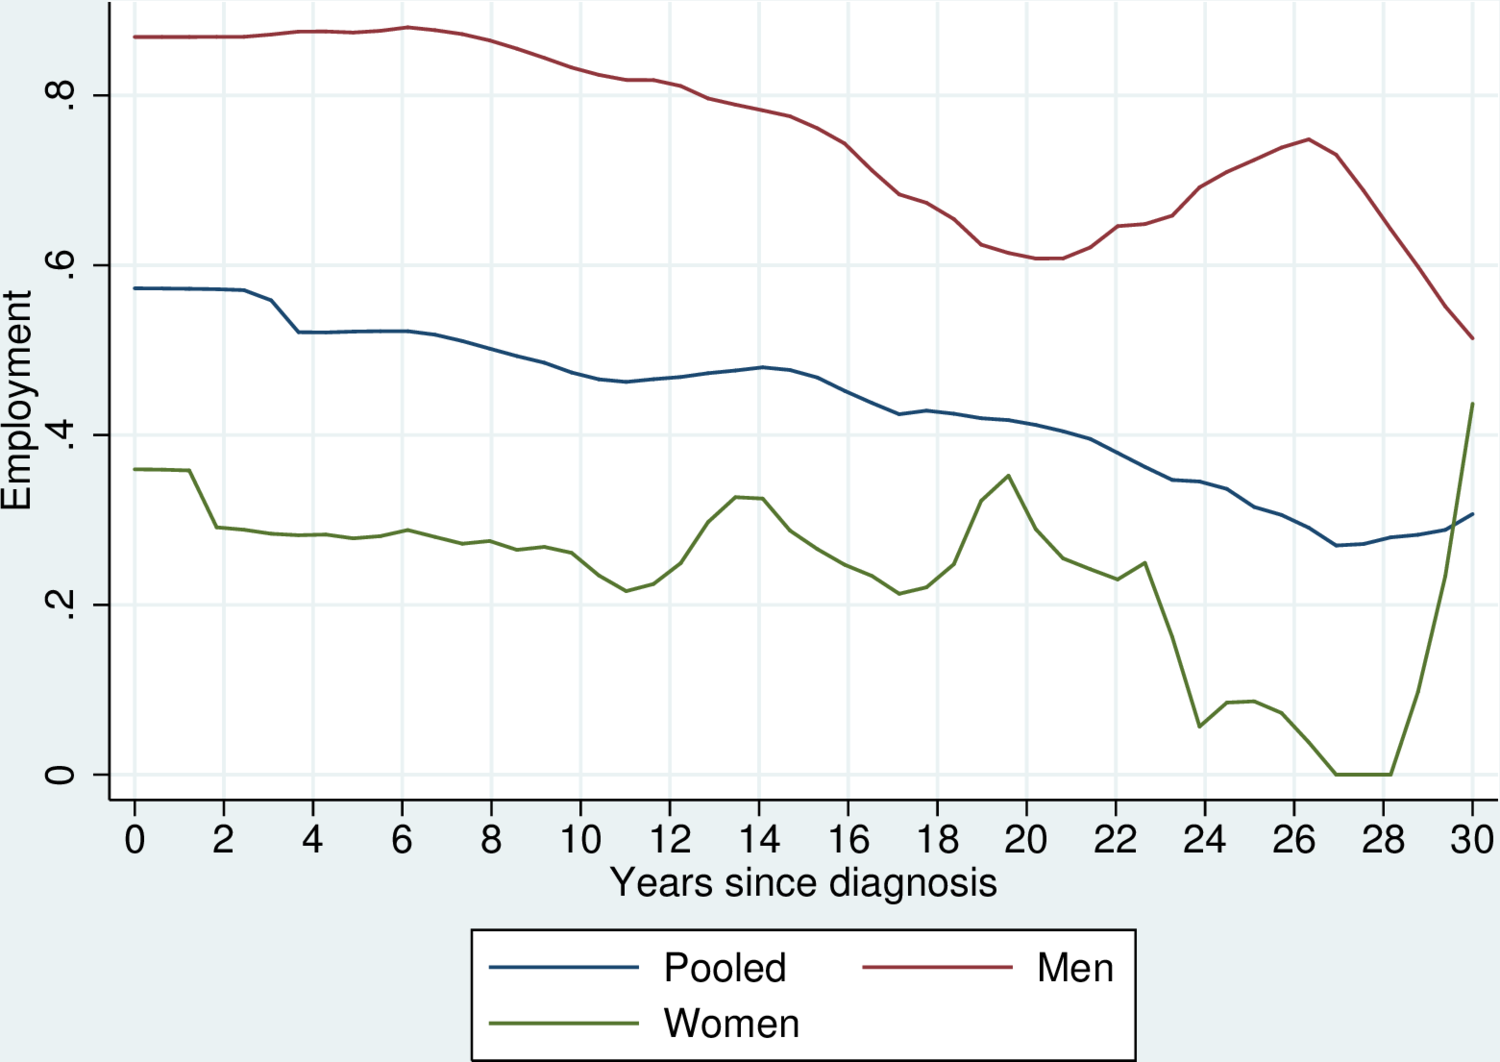
\includegraphics[width=0.7\columnwidth]{figures/lpoly_works_diabetesduration/lpoly_works_diabetesduration}
\end{center}
\end{figure}

\begin{figure}[h!]
\caption{\label{fig:Kernel-weighted-local-polynomial_wage}Kernel-weighted local
polynomial regression of log hourly wages on diabetes duration}%
\begin{center}
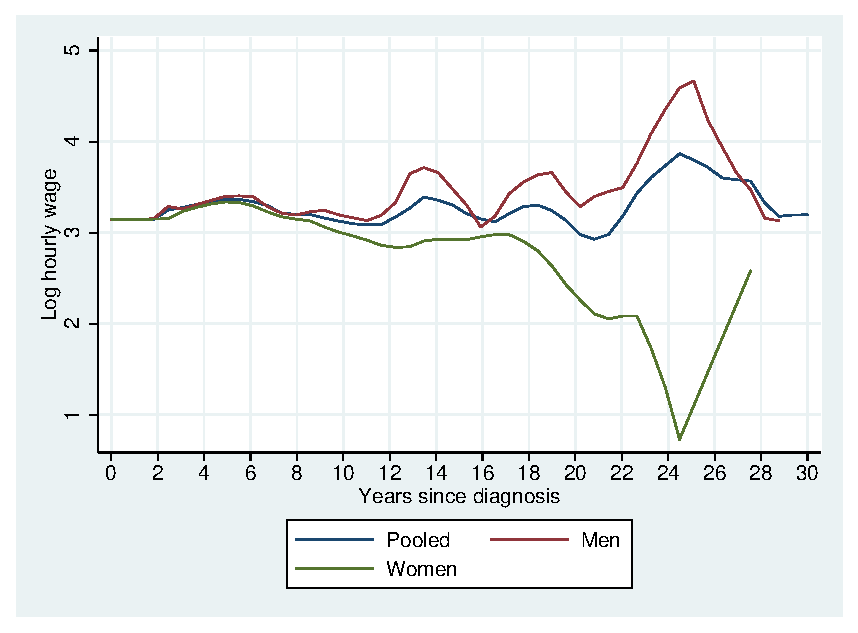
\includegraphics[width=0.7\columnwidth]{figures/lpoly_wage_diabetesduration/lpoly_wage_diabetesduration}
\end{center}
\end{figure}

\begin{figure}[h!]
\caption{\label{fig:Kernel-weighted-local-polynomial_workhrs}Kernel-weighted local
polynomial regression of working hours on diabetes duration}%
\begin{center}
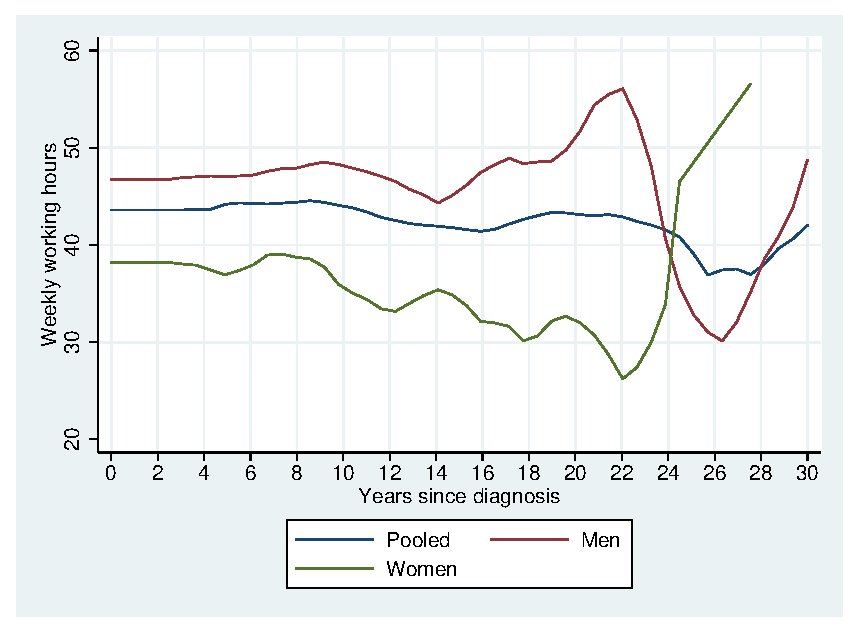
\includegraphics[width=0.7\columnwidth]{figures/lpoly_workhrs_diabetesduration/lpoly_workhrs_diabetesduration}
\end{center}
\end{figure}

\FloatBarrier

First, models with a linear diabetes duration specification are presented
in table \ref{tab:Self-reported-diabetes-duration-linear}. The results
indicate a reduction of about 1.8 percentage points for men with each
additional year since diagnosis. For women the coefficient shows a
reduction of about one percentage point per year\DIFaddbegin \DIFadd{, }\DIFaddend though the association
is not as strong. Interestingly, we find a reduction in female wages of about seven percentage points per year with diabetes but no effects for males and for the working hour models.
\begin{table}[h]
\caption{\label{tab:Self-reported-diabetes-duration-linear}Relationship of self-reported years since diagnosis and labor market outcomes}
\begin{center}
%\resizebox{\textwidth}{!}{%
\begin{adjustbox}{max width=\textwidth}

{
\def\sym#1{\ifmmode^{#1}\else\(^{#1}\)\fi}
\begin{tabular}{l*{9}{SS}}
\toprule
                &\multicolumn{3}{c}{Employment}                          &\multicolumn{3}{c}{Log monthly wages}                   &\multicolumn{3}{c}{Monthly work hours}                  \\\cmidrule(lr){2-4}\cmidrule(lr){5-7}\cmidrule(lr){8-10}
                &\multicolumn{1}{c}{(1)}&\multicolumn{1}{c}{(2)}&\multicolumn{1}{c}{(3)}&\multicolumn{1}{c}{(4)}&\multicolumn{1}{c}{(5)}&\multicolumn{1}{c}{(6)}&\multicolumn{1}{c}{(7)}&\multicolumn{1}{c}{(8)}&\multicolumn{1}{c}{(9)}\\
                &\multicolumn{1}{c}{Pooled}&\multicolumn{1}{c}{Males}&\multicolumn{1}{c}{Females}&\multicolumn{1}{c}{Pooled}&\multicolumn{1}{c}{Males}&\multicolumn{1}{c}{Females}&\multicolumn{1}{c}{Pooled}&\multicolumn{1}{c}{Males}&\multicolumn{1}{c}{Females}\\
\midrule
\multicolumn{10}{l}{ \textit{Fixed Effects}}\\
Diabetes duration&    -.013\sym{***}&    -.018\sym{***}&    -.011\sym{**} &    -.028\sym{*}  &    -.018         &    -.069\sym{**} &     .125         &     .167         &     .094         \\
                &   (.004)         &   (.006)         &   (.005)         &   (.016)         &   (.018)         &   (.029)         &   (.316)         &   (.353)         &   (.679)         \\
\midrule
\multicolumn{10}{l}{ \textit{Random Effects}}\\
Diabetes duration&    -.013\sym{***}&    -.011\sym{***}&    -.008\sym{***}&    -.002         &     .007         &    -.013         &    -.086         &    -.064         &    -.136         \\
                &   (.004)         &   (.002)         &   (.001)         &   (.004)         &   (.005)         &   (.009)         &   (.083)         &   (.103)         &   (.129)         \\
\midrule
N               &    38398         &    16073         &    22325         &    16288         &    10604         &     5684         &    20691         &    13375         &     7316         \\
\bottomrule
\multicolumn{10}{l}{\footnotesize Robust standard errors in parentheses}\\
\multicolumn{10}{l}{\footnotesize Other control variables: state dummies, urbanization dummies, education dummies, married dummy, number children < 6}\\
\multicolumn{10}{l}{\footnotesize wealth, age and calender year fixed effects}\\
\multicolumn{10}{l}{\footnotesize The random effects model additionally controls for initial age when entering the survey, being indigenous and gender}\\
\multicolumn{10}{l}{\footnotesize The wage and working hour models additionally control for type of work (agricultural and self employed with}\\
\multicolumn{10}{l}{\footnotesize non-agricultural employment as the base) and for health insurance status}\\
\multicolumn{10}{l}{\footnotesize \sym{*} \(p<0.10\), \sym{**} \(p<0.05\), \sym{***} \(p<0.01\)}\\
\end{tabular}
}
%}

\end{adjustbox}
\end{center}
\end{table}  

  
  
Using the non-linear specification with splines, we find that for the pooled sample employment chances
are mainly reduced for those reporting a diagnosis more than eleven years
ago, with each additional year reducing employment chances by about
two percentage points (Table \ref{tab:Self-reported-diabetes-duration-splines-1}).
When stratified by gender, the
negative association persists for males and females, albeit much \DIFdelbegin \DIFdel{weaker }\DIFdelend \DIFaddbegin \DIFadd{more weakly }\DIFaddend for the latter. Interestingly, using splines
we find a relatively strong reduction of wages 5-11 years after diagnosis
for women. We also find some significant associations for those with more than 20 years of diabetes\DIFdelbegin \DIFdel{, however}\DIFdelend \DIFaddbegin \DIFadd{. However}\DIFaddend , these estimates are likely spurious due to the considerably reduced number of observations\DIFaddbegin \DIFadd{, }\DIFaddend particularly for wages and working hours.

\begin{table}[h]
\caption{\label{tab:Self-reported-diabetes-duration-splines-1}Relationship
of self-reported years since diagnosis and labor market outcomes
using linear splines }
%\resizebox{\textwidth}{!}{%
\begin{center}
\begin{adjustbox}{max width=\textwidth}

{
\def\sym#1{\ifmmode^{#1}\else\(^{#1}\)\fi}
\begin{tabular}{l*{9}{SS}}
\toprule
                &\multicolumn{3}{c}{Employment}                          &\multicolumn{3}{c}{Log monthly wages}                   &\multicolumn{3}{c}{Monthly work hours}                  \\\cmidrule(lr){2-4}\cmidrule(lr){5-7}\cmidrule(lr){8-10}
                &\multicolumn{1}{c}{(1)}&\multicolumn{1}{c}{(2)}&\multicolumn{1}{c}{(3)}&\multicolumn{1}{c}{(4)}&\multicolumn{1}{c}{(5)}&\multicolumn{1}{c}{(6)}&\multicolumn{1}{c}{(7)}&\multicolumn{1}{c}{(8)}&\multicolumn{1}{c}{(9)}\\
                &\multicolumn{1}{c}{Pooled}&\multicolumn{1}{c}{Males}&\multicolumn{1}{c}{Females}&\multicolumn{1}{c}{Pooled}&\multicolumn{1}{c}{Males}&\multicolumn{1}{c}{Females}&\multicolumn{1}{c}{Pooled}&\multicolumn{1}{c}{Males}&\multicolumn{1}{c}{Females}\\
\midrule
\multicolumn{10}{l}{\hspace*{50mm}\textit{Fixed Effects}}\\
\multicolumn{10}{l}{Years since diagnosis}\\
\hspace*{10mm}0--4&    -.018\sym{*}  &    -.017         &    -.018         &    -.009         &    -.022         &     .037         &     .592         &     .430         &    1.499         \\
                &   (.010)         &   (.013)         &   (.015)         &   (.044)         &   (.047)         &   (.116)         &   (.841)         &   (.880)         &  (2.306)         \\
\hspace*{10mm}5--11&    -.005         &    -.008         &    -.005         &    -.052\sym{*}  &    -.038         &    -.112\sym{**} &    -.150         &     .005         &    -.536         \\
                &   (.006)         &   (.009)         &   (.008)         &   (.031)         &   (.036)         &   (.050)         &   (.524)         &   (.602)         &  (1.016)         \\
\hspace*{10mm}12--20&    -.024\sym{***}&    -.036\sym{**} &    -.017\sym{*}  &     .018         &     .052         &    -.045         &    -.011         &     .158         &    -.738         \\
                &   (.009)         &   (.017)         &   (.010)         &   (.049)         &   (.063)         &   (.055)         &   (.811)         &   (.977)         &  (1.501)         \\
\hspace*{10mm}> 20&    -.021         &    -.024         &    -.019         &    -.064         &    -.006         &    -.212\sym{***}&    1.986         &     .770         &    8.291\sym{***}\\
                &   (.017)         &   (.040)         &   (.018)         &   (.123)         &   (.124)         &   (.058)         &  (3.363)         &  (3.439)         &  (1.832)         \\
\midrule
\multicolumn{10}{l}{\hspace*{50mm}\textit{Random Effects}}\\
\multicolumn{10}{l}{Years since diagnosis}\\
\hspace*{10mm}0--4&    -.026\sym{***}&    -.012\sym{*}  &    -.021\sym{***}&     .024\sym{*}  &     .027\sym{*}  &     .027         &     .102         &    -.127         &     .493         \\
                &   (.005)         &   (.006)         &   (.006)         &   (.014)         &   (.016)         &   (.027)         &   (.296)         &   (.341)         &   (.574)         \\
\hspace*{10mm}5--11&    -.002         &    -.005         &    -.000         &    -.031\sym{**} &    -.023         &    -.048\sym{**} &    -.107         &     .007         &    -.356         \\
                &   (.005)         &   (.007)         &   (.006)         &   (.015)         &   (.018)         &   (.024)         &   (.321)         &   (.394)         &   (.544)         \\
\hspace*{10mm}12--20&    -.018\sym{***}&    -.023\sym{**} &    -.009         &    -.002         &     .027         &    -.065\sym{*}  &    -.116         &     .022         &    -.368         \\
                &   (.006)         &   (.010)         &   (.007)         &   (.025)         &   (.031)         &   (.039)         &   (.428)         &   (.572)         &   (.726)         \\
\hspace*{10mm}> 20&    -.006         &    -.009         &    -.002         &     .027\sym{**} &     .033         &     .041\sym{***}&    -.470         &    -.569         &    -.330         \\
                &   (.004)         &   (.008)         &   (.004)         &   (.012)         &   (.044)         &   (.015)         &   (.310)         &  (1.191)         &   (.321)         \\
N               &    38398         &    16073         &    22325         &    16288         &    10604         &     5684         &    20691         &    13375         &     7316         \\
\bottomrule
\multicolumn{10}{l}{\footnotesize Robust standard errors in parentheses}\\
\multicolumn{10}{l}{\footnotesize Other control variables: state dummies, urbanization dummies, education dummies, married dummy, number children < 6}\\
\multicolumn{10}{l}{\footnotesize wealth, age and calender year fixed effects}\\
\multicolumn{10}{l}{\footnotesize The random effects model additionally controls for initial age when entering the survey, being indigenous and gender}\\
\multicolumn{10}{l}{\footnotesize The wage and working hour models additionally control for type of work (agricultural and self employed with}\\
\multicolumn{10}{l}{\footnotesize non-agricultural employment as the base) and for health insurance status}\\
\multicolumn{10}{l}{\footnotesize \sym{*} \(p<0.10\), \sym{**} \(p<0.05\), \sym{***} \(p<0.01\)}\\
\end{tabular}
}
\end{adjustbox}
\end{center}
\end{table}

Overall, the duration results are somewhat different to those found by \citet{Minor2013} for the \ac{USA}, who does not find evidence for a linear relationship of diabetes duration with employment chances. Our results from the non-linear analysis are not directly comparable as \citet{Minor2013} uses dummy variables to identify different diabetes durations. Nonetheless, they are similar in that he does not find an immediate effect of a diabetes diagnosis on employment chances. However, the effects still appear at an earlier point than in our analysis and are in general much larger. However, apart from not using splines he does not use individual fixed effects so that his results might suffer from bias leading to the larger effect sizes\DIFdelbegin \DIFdel{or }\DIFdelend \DIFaddbegin \DIFadd{. It may of course also be that }\DIFaddend the effects of diabetes in the \ac{USA} are simply \DIFdelbegin \DIFdel{much larger }\DIFdelend \DIFaddbegin \DIFadd{larger than in Mexico}\DIFaddend .

As a robustness check and due to the reduced number of observations for twenty or more years with diabetes we estimated the linear model again excluding those above nineteen years of diabetes to investigate if the effects were driven by these rare observations. These results are available on request and indicate marginally smaller effect sizes, but do not change the qualitative interpretation of the effects.

Generally, the results so far have revealed an important adverse association of self-reported diabetes with employment chances for men\DIFdelbegin \DIFdel{and also has }\DIFdelend \DIFaddbegin \DIFadd{; the findings have also }\DIFaddend provided additional evidence of adverse effects for females, supporting earlier findings for Mexico \DIFdelbegin \DIFdel{.}\DIFdelend \DIFaddbegin \DIFadd{\mbox{%DIFAUXCMD
\citep{Seuring2015}
}%DIFAUXCMD
.}\DIFaddend \footnote{As  a robustness check of our results of the linear probability model for employment status, we also estimated \DIFaddbegin \DIFadd{a }\DIFaddend population-averaged panel-data model with the probit link function. To account for fixed unobserved heterogeneity in this type of model we used the 'within-between' formulation proposed by \citet{Bell2015} based on the work of \citet{Mundlak1978}, which allows to account for \DIFdelbegin \DIFdel{time-constant }\DIFdelend \DIFaddbegin \DIFadd{time-invariant }\DIFaddend unobserved heterogeneity by adding the individual group means as regressors. The 'within-between' formulation also adds group means but uses the demeaned values instead of the complete observation to capture any within variation. This has some advantages as it allows to differentiate clearly between the within and the between effects of the used variables and is less prone to issues of collinearity and multicollinearity. Using this
strategy has yielded qualitatively similar results to those of the
linear fixed effects specifications\DIFdelbegin \DIFdel{and the }\DIFdelend \DIFaddbegin \DIFadd{. The }\DIFaddend results are available
on request \DIFaddbegin \DIFadd{from the authors}\DIFaddend .} We only find very limited evidence for any relationship of self reported diabetes with wages or working hours \DIFdelbegin \DIFdel{which is }\DIFdelend \DIFaddbegin \DIFadd{- }\DIFaddend in line with the results of \citet{Minor2013}, who does not find strong evidence for any effects beyond those on employment, though he does not look at working hours. Reasons for this difference in effects at the extensive and intensive margin might be that people who are diagnosed while employed are able to continue to work if they do not suffer from any severe complications yet. They also may resort to doing different activities within the workplace that are less physically demanding and allow them to continue working and earning similar wages as before their diagnosis. Only once complications become increasingly severe \DIFaddbegin \DIFadd{would }\DIFaddend they drop out of the labor market\DIFaddbegin \DIFadd{, }\DIFaddend without going through a previous phase of reduced productivity and labor supply. Some support for this reasoning comes from the \ac{RE} results in tables \ref{tab:Self-reported-diabetes-and} and \ref{tab:Self-reported-diabetes-interaction}\DIFdelbegin \DIFdel{that show }\DIFdelend \DIFaddbegin \DIFadd{, showing }\DIFaddend that people with diabetes still employed actually earn more if we disregard any unobserved selection into employment, i.e\DIFaddbegin \DIFadd{. }\DIFaddend those with diabetes that are able to remain employed have some unobserved characteristics that also allow them to earn higher wages. These people might have abilities that make them better at managing their diabetes and also lets them earn higher wages\DIFaddbegin \DIFadd{, }\DIFaddend or they may be so valuable to their working environment that they do not lose their job even if they are \DIFdelbegin \DIFdel{limited healthwise }\DIFdelend \DIFaddbegin \DIFadd{constraint health-wise }\DIFaddend due to diabetes. This \DIFdelbegin \DIFdel{appears }\DIFdelend \DIFaddbegin \DIFadd{seems }\DIFaddend to be particularly the case for those in non-agricultural employment. Overall, it appears that diabetes affects those self-employed or in agricultural employment much more, potentially because they often cannot rely on formal contracts that would protect them against job loss, they are likely less able to access appropriate treatment or are diagnosed much later also due to a lack of access to proper health care\DIFaddbegin \DIFadd{, }\DIFaddend leading to a more rapid development of diabetes complications and also because their jobs are likely more physically demanding, making it harder to continue working once complications appear. However, this reasoning remains \DIFaddbegin \DIFadd{somewhat }\DIFaddend speculative and deserves further research in future studies.

Finally, before moving on to further analysis, we \DIFdelbegin \DIFdel{want to note }\DIFdelend \DIFaddbegin \DIFadd{need to emphasise }\DIFaddend that our fixed effects strategy used to identify the effect of self-reported diabetes relies on those reporting a new diabetes diagnosis between any of the waves, which disregards people that have had diabetes before the start of the survey and so limits the estimation of effects to those more or less recently diagnosed. Accordingly, the obtained results may be different from those with a longer disease history. However, at least the results of the \ac{RE} analysis, which also includes \DIFdelbegin \DIFdel{between person }\DIFdelend \DIFaddbegin \DIFadd{between-person }\DIFaddend variation, do not indicate that the effects are substantially different even when people with a longer disease history are taken into account. We have to note nonetheless that the analysis of diabetes duration shows somewhat different results \DIFdelbegin \DIFdel{with regards to }\DIFdelend \DIFaddbegin \DIFadd{in terms of }\DIFaddend when the adverse effects appear, as it indicates that the largest effects are found for those with a disease duration over 10 years\DIFaddbegin \DIFadd{, }\DIFaddend which would suggest no immediate effect of diabetes. \DIFdelbegin \DIFdel{However, and }\DIFdelend \DIFaddbegin \DIFadd{Yet, }\DIFaddend as we have mentioned before, the duration analysis relies on information only from the most recent wave to construct a measure of disease duration for all previous waves and hence excludes information from participants dropping out of the sample before the last wave. It further relies on people correctly identifying the year of first diagnosis which is likely subject to recall bias\DIFaddbegin \DIFadd{, }\DIFaddend the longer the diagnosis lies in the past, so that the results might not be directly comparable and generally less reliable than the estimates using self-reported diabetes from all three waves. Also, given that the signs point \DIFdelbegin \DIFdel{toward }\DIFdelend \DIFaddbegin \DIFadd{towards }\DIFaddend a negative effect also immediately after diagnosis (which is also supported by the \ac{RE} results), but standard errors are \DIFdelbegin \DIFdel{to }\DIFdelend \DIFaddbegin \DIFadd{too }\DIFaddend large to suggest statistical significance\DIFdelbegin \DIFdel{could be a result of }\DIFdelend \DIFaddbegin \DIFadd{, this hints at }\DIFaddend a lack of statistical power to identify a relationship for the other duration groups in the analysis using splines. Accordingly, further research in this area is needed to better understand when adverse effects appear. [NOT SURE IF THIS PARA SHOULD BE INCLUDED AS IT PARTICULALRY QUESTIONS THE RESULTS OF THE DURATION ANALYSIS. WHAT DO YOU THINK? ]


\subsection{Cross-sectional biomarker analysis}

The results presented in the previous section did provide important
information on the association between self-reported diabetes and
\DIFdelbegin \DIFdel{with }\DIFdelend labor market outcomes in Mexico.

While panel data methods have obvious advantages over a cross sectional
analysis, there are additional insights
to be gained from making use of the biomarker data collected in the
third wave of the \ac{MxFLS}, even if it only allows for a cross-sectional
analysis. The biomarker data allows us to identify respondents with
\ac{HbA1c} levels, thereby identifying diabetes cases that have
not yet been 'officially' diagnosed. As mentioned before, biomarker
data are only available for a subsample of the survey, including everybody
aged 45+ as well as a random selection of participants below age 45
\citep{Crimmins2015}. In this sub-sample 694 (10 percent) self-report
diabetes and 1,248 (18 percent) have undiagnosed diabetes, i.e. as
measured by an \ac{HbA1c} equal to or greater than 6.5 percent. In an effort to reduce bias in our estimates we additionally estimate every model using community fixed effects to account for unobserved community characteristics\DIFaddbegin \DIFadd{, }\DIFaddend such as the access to healthcare and the quality of healthcare in the community, poverty and unemployment levels in the community or the amount of public green space and recreational possibilities available. These factors could potentially affect the propensity to \DIFdelbegin \DIFdel{develop diabetes as well as }\DIFdelend \DIFaddbegin \DIFadd{(1) develop diabetes and (2) }\DIFaddend to receive a diagnosis of diabetes\DIFdelbegin \DIFdel{and might also }\DIFdelend \DIFaddbegin \DIFadd{, plus they might }\DIFaddend affect labor market outcomes.\footnote{We did not use household fixed effects as the \DIFaddbegin \DIFadd{average }\DIFaddend number of observations per household was close to one\DIFaddbegin \DIFadd{, i.e. for most households only one member provided biomarker information in our subsample,  }\DIFaddend significantly limiting the variation within households \DIFaddbegin \DIFadd{that would be }\DIFaddend needed for identification.}


\subsubsection*{Ojectively measured diabetes}


The results of the complete biomarker analysis are presented in table \ref{tab:Biomarker_results}. In order to investigate how the subsample of biomarkers compares to the overall sample of the third wave we first estimate a model showing the association of self-reported diabetes with our outcome variables using data of the entire third wave (columns 1--3 and 13--15 in table \ref{tab:Biomarker_results}). We find similar results to our panel data analysis\DIFdelbegin \DIFdel{albeit }\DIFdelend \DIFaddbegin \DIFadd{, if }\DIFaddend with somewhat smaller coefficients for the effect on employment chances, particularly for females\DIFdelbegin \DIFdel{, suggesting }\DIFdelend \DIFaddbegin \DIFadd{. This suggests }\DIFaddend that not accounting for fixed effects might underestimate the effect of self-reported diabetes on women employment chance. Running the same model but using only the data of the biomarker sample (columns 4--6 and 16--18), we find that the coefficient becomes smaller for men and standard \DIFdelbegin \DIFdel{increase throughout likely die }\DIFdelend \DIFaddbegin \DIFadd{errors increase throughout, likely due }\DIFaddend to the reduction in sample size. This \DIFdelbegin \DIFdel{suggests }\DIFdelend \DIFaddbegin \DIFadd{indicates }\DIFaddend that the oversampling of older people in the subsample may \DIFdelbegin \DIFdel{introduces }\DIFdelend \DIFaddbegin \DIFadd{introduce }\DIFaddend a downward bias in the estimates for males\DIFaddbegin \DIFadd{, }\DIFaddend which has to be taken into account when interpreting the results.

In the next step we investigate the association between objectively measured
diabetes, irrespective of whether
the condition has or has not been diagnosed, and labor market outcomes\DIFaddbegin \DIFadd{, }\DIFaddend by estimating equation \ref{eq:diab_objective}. \footnote{The diabetes indicator
variable still also contains those that self-reported a diabetes diagnosis
but had \ac{HbA1c} levels below the diabetes threshold. This is sensible as it is possible that people with a diabetes diagnosis are able to manage their diabetes in such a way that their \ac{HbA1c} drop below the threshold and should not be assumed to having falsely reported a diabetes diagnosis \DIFdelbegin \DIFdel{, albeit }\DIFdelend \DIFaddbegin \DIFadd{(even though }\DIFaddend this \DIFdelbegin \DIFdel{admittedly is a possibility as well}\DIFdelend \DIFaddbegin \DIFadd{could potentially also be the case)}\DIFaddend . Robustness checks where we specifically accounted for this subpopulation
did not show qualitatively different results.}  We find an adverse association of objectively measured diabetes and employment
chances for the pooled (columns 7--9) and to some \DIFdelbegin \DIFdel{extend }\DIFdelend \DIFaddbegin \DIFadd{extent }\DIFaddend for the female sample (columns 19--21), but the coefficient size is reduced throughout\DIFaddbegin \DIFadd{, }\DIFaddend compared to self-reported diabetes. This suggests that relying on self-reported
diabetes exclusively may lead to an upward bias due to those undiagnosed experiencing less pronounced adverse labor market effects.
To further investigate this, we include both diagnosed and undiagnosed diabetes jointly as independent explanatory variables\DIFaddbegin \DIFadd{, }\DIFaddend to account for the differences between the two groups as in equation \ref{eq:diab_sr_ud}.

As shown in columns 10--12 and 22--24, no association between undiagnosed
diabetes and any labor outcome is found. For those with diagnosed
diabetes the coefficients for the association with employment chances
 for the pooled sample and women are similar in size and significance to those of the panel analysis, particularly when we include community level fixed effects. They also do not differ much from the results of the specification only accounting for self-reported diabetes. Consistent with our earlier findings there is no indication of any associations between any form of diabetes and wages or working hours. 


\setlength{\tabcolsep}{0pt}
\begin{landscape}
\begin{table}
\caption{\label{tab:Biomarker_results}Biomarker results}
\begin{center}
\begin{adjustbox}{max width=\linewidth}
{
\def\sym#1{\ifmmode^{#1}\else\(^{#1}\)\fi}
\begin{tabular}{l*{24}{SS}}
\toprule
                &\multicolumn{3}{c}{SR (complete sample)}&\multicolumn{3}{c}{SR (biomarker sample)}&\multicolumn{3}{c}{HbA1c $\geq 6.5\%$}                  &\multicolumn{3}{c}{SR and undiagnosed}       &\multicolumn{3}{c}{SR (complete sample) (FE)}&\multicolumn{3}{c}{SR (biomarker sample) (FE)}&\multicolumn{3}{c}{HbA1c $\geq 6.5\%$ (FE)}             &\multicolumn{3}{c}{SR and undiagnosed (FE)}  \\\cmidrule(lr){2-4}\cmidrule(lr){5-7}\cmidrule(lr){8-10}\cmidrule(lr){11-13}\cmidrule(lr){14-16}\cmidrule(lr){17-19}\cmidrule(lr){20-22}\cmidrule(lr){23-25}
                &\multicolumn{1}{c}{(1)}&\multicolumn{1}{c}{(2)}&\multicolumn{1}{c}{(3)}&\multicolumn{1}{c}{(4)}&\multicolumn{1}{c}{(5)}&\multicolumn{1}{c}{(6)}&\multicolumn{1}{c}{(7)}&\multicolumn{1}{c}{(8)}&\multicolumn{1}{c}{(9)}&\multicolumn{1}{c}{(10)}&\multicolumn{1}{c}{(11)}&\multicolumn{1}{c}{(12)}&\multicolumn{1}{c}{(13)}&\multicolumn{1}{c}{(14)}&\multicolumn{1}{c}{(15)}&\multicolumn{1}{c}{(16)}&\multicolumn{1}{c}{(17)}&\multicolumn{1}{c}{(18)}&\multicolumn{1}{c}{(19)}&\multicolumn{1}{c}{(20)}&\multicolumn{1}{c}{(21)}&\multicolumn{1}{c}{(22)}&\multicolumn{1}{c}{(23)}&\multicolumn{1}{c}{(24)}\\
                &\multicolumn{1}{c}{Pooled}&\multicolumn{1}{c}{Males}&\multicolumn{1}{c}{Females}&\multicolumn{1}{c}{Pooled}&\multicolumn{1}{c}{Males}&\multicolumn{1}{c}{Females}&\multicolumn{1}{c}{Pooled}&\multicolumn{1}{c}{Males}&\multicolumn{1}{c}{Females}&\multicolumn{1}{c}{Pooled}&\multicolumn{1}{c}{Males}&\multicolumn{1}{c}{Females}&\multicolumn{1}{c}{Pooled}&\multicolumn{1}{c}{Males}&\multicolumn{1}{c}{Females}&\multicolumn{1}{c}{Pooled}&\multicolumn{1}{c}{Males}&\multicolumn{1}{c}{Females}&\multicolumn{1}{c}{Pooled}&\multicolumn{1}{c}{Males}&\multicolumn{1}{c}{Females}&\multicolumn{1}{c}{Pooled}&\multicolumn{1}{c}{Males}&\multicolumn{1}{c}{Females}\\
\midrule
\multicolumn{25}{l}{\hspace*{10mm}\textbf{Dependent variable: Employment}} \\
\addlinespace 
Diagnosed diabetes&    -.062\sym{***}&    -.058\sym{***}&    -.044\sym{**} &    -.057\sym{***}&    -.042         &    -.041\sym{*}  &                  &                  &                  &    -.058\sym{***}&    -.041         &    -.043\sym{*}  &    -.066\sym{***}&    -.068\sym{***}&    -.046\sym{***}&    -.060\sym{***}&    -.050\sym{*}  &    -.043\sym{*}  &                  &                  &                  &    -.063\sym{***}&    -.049\sym{*}  &    -.048\sym{**} \\
                &   (.013)         &   (.018)         &   (.017)         &   (.017)         &   (.026)         &   (.022)         &                  &                  &                  &   (.017)         &   (.026)         &   (.023)         &   (.012)         &   (.017)         &   (.017)         &   (.017)         &   (.026)         &   (.023)         &                  &                  &                  &   (.018)         &   (.026)         &   (.023)         \\
HbA1c $\geq 6.5\%$&                  &                  &                  &                  &                  &                  &    -.023\sym{**} &    -.009         &    -.021 &                  &                  &                  &                  &                  &                  &                  &                  &                  &    -.032\sym{***}&    -.013         &    -.032\sym{*}&                  &                  &                  \\
                &                  &                  &                  &                  &                  &                  &   (.012)         &   (.015)         &   (.017)         &                  &                  &                  &                  &                  &                  &                  &                  &                  &   (.012)         &   (.015)         &   (.018)         &                  &                  &                  \\
Undiagnosed diabetes&                  &                  &                  &                  &                  &                  &                  &                  &                  &    -.004         &     .006         &    -.008         &                  &                  &                  &                  &                  &                  &                  &                  &                  &    -.013         &     .005         &    -.018         \\
                &                  &                  &                  &                  &                  &                  &                  &                  &                  &   (.014)         &   (.016)         &   (.020)         &                  &                  &                  &                  &                  &                  &                  &                  &                  &   (.014)         &   (.019)         &   (.018)         \\
\midrule
R2              &\multicolumn{1}{S}{.307}         &\multicolumn{1}{S}{.095}         &\multicolumn{1}{S}{.143}         &\multicolumn{1}{S}{.326}         &\multicolumn{1}{S}{.086}         &\multicolumn{1}{S}{.151}         &\multicolumn{1}{S}{.326}         &\multicolumn{1}{S}{.085}         &\multicolumn{1}{S}{.326}         &\multicolumn{1}{S}{.326}         &\multicolumn{1}{S}{.086}         &\multicolumn{1}{S}{.151}         &\multicolumn{1}{S}{.302}         &\multicolumn{1}{S}{.093}         &\multicolumn{1}{S}{.104}         &\multicolumn{1}{S}{.328}         &\multicolumn{1}{S}{.082}         &\multicolumn{1}{S}{.108}         &\multicolumn{1}{S}{.328}         &\multicolumn{1}{S}{.080}         &\multicolumn{1}{S}{.328}         &\multicolumn{1}{S}{.328}         &\multicolumn{1}{S}{.082}         &\multicolumn{1}{S}{.108}         \\
N               &\multicolumn{1}{c}{18748}         &\multicolumn{1}{c}{8234}         &\multicolumn{1}{c}{10514}         &\multicolumn{1}{c}{6408}         &\multicolumn{1}{c}{2785}         &\multicolumn{1}{c}{3623}         &\multicolumn{1}{c}{6416}         &\multicolumn{1}{c}{2790}         &\multicolumn{1}{c}{3623}         &\multicolumn{1}{c}{6408}         &\multicolumn{1}{c}{2785}         &\multicolumn{1}{c}{3623}         &\multicolumn{1}{c}{18748}         &\multicolumn{1}{c}{8234}         &\multicolumn{1}{c}{10514}         &\multicolumn{1}{c}{6408}         &\multicolumn{1}{c}{2785}         &\multicolumn{1}{c}{3623}         &\multicolumn{1}{c}{6416}         &\multicolumn{1}{c}{2790}         &\multicolumn{1}{c}{6416}         &\multicolumn{1}{c}{6408}         &\multicolumn{1}{c}{2785}         &\multicolumn{1}{c}{3623}         \\
\midrule
\multicolumn{19}{l}{\hspace*{10mm}\textbf{Dependent variable: Log hourly wages}} \\ 
\addlinespace
Diagnosed diabetes&    -.002         &     .034         &    -.054         &     .012         &     .021         &     .004         &                  &                  &                  &     .001         &     .007         &     .006         &     .004         &     .043         &    -.048         &     .003         &    -.008         &    -.039         &                  &                  &                  &     .006         &    -.004         &    -.051         \\
                &   (.039)         &   (.044)         &   (.072)         &   (.053)         &   (.062)         &   (.101)         &                  &                  &                  &   (.054)         &   (.064)         &   (.104)         &   (.038)         &   (.047)         &   (.072)         &   (.053)         &   (.066)         &   (.113)         &                  &                  &                  &   (.056)         &   (.068)         &   (.117)         \\
HbA1c $\geq 6.5\%$&                  &                  &                  &                  &                  &                  &    -.025         &    -.027         &    -.025         &                  &                  &                  &                  &                  &                  &                  &                  &                  &     .009         &     .011         &     .009         &                  &                  &                  \\
                &                  &                  &                  &                  &                  &                  &   (.034)         &   (.040)         &   (.034)         &                  &                  &                  &                  &                  &                  &                  &                  &                  &   (.036)         &   (.044)         &   (.036)         &                  &                  &                  \\
Undiagnosed diabetes&                  &                  &                  &                  &                  &                  &                  &                  &                  &    -.029         &    -.035         &    -.036         &                  &                  &                  &                  &                  &                  &                  &                  &                  &     .012         &     .018         &    -.052         \\
                &                  &                  &                  &                  &                  &                  &                  &                  &                  &   (.039)         &   (.045)         &   (.072)         &                  &                  &                  &                  &                  &                  &                  &                  &                  &   (.039)         &   (.048)         &   (.079)         \\
\midrule
R2              &\multicolumn{1}{S}{.221}         &\multicolumn{1}{S}{.206}         &\multicolumn{1}{S}{.264}         &\multicolumn{1}{S}{.257}         &\multicolumn{1}{S}{.246}         &\multicolumn{1}{S}{.312}         &\multicolumn{1}{S}{.258}         &\multicolumn{1}{S}{.246}         &\multicolumn{1}{S}{.258}         &\multicolumn{1}{S}{.266}         &\multicolumn{1}{S}{.255}         &\multicolumn{1}{S}{.326}         &\multicolumn{1}{S}{.141}         &\multicolumn{1}{S}{.117}         &\multicolumn{1}{S}{.183}         &\multicolumn{1}{S}{.170}         &\multicolumn{1}{S}{.146}         &\multicolumn{1}{S}{.236}         &\multicolumn{1}{S}{.171}         &\multicolumn{1}{S}{.146}         &\multicolumn{1}{S}{.171}         &\multicolumn{1}{S}{.170}         &\multicolumn{1}{S}{.146}         &\multicolumn{1}{S}{.237}         \\
N               &\multicolumn{1}{c}{8402}         &\multicolumn{1}{c}{5515}         &\multicolumn{1}{c}{2887}         &\multicolumn{1}{c}{2687}         &\multicolumn{1}{c}{1803}         &\multicolumn{1}{c}{884}         &\multicolumn{1}{c}{2690}         &\multicolumn{1}{c}{1805}         &\multicolumn{1}{c}{2690}         &\multicolumn{1}{c}{2687}         &\multicolumn{1}{c}{1803}         &\multicolumn{1}{c}{884}         &\multicolumn{1}{c}{8402}         &\multicolumn{1}{c}{5515}         &\multicolumn{1}{c}{2887}         &\multicolumn{1}{c}{2687}         &\multicolumn{1}{c}{1803}         &\multicolumn{1}{c}{884}         &\multicolumn{1}{c}{2690}         &\multicolumn{1}{c}{1805}         &\multicolumn{1}{c}{2690}         &\multicolumn{1}{c}{2687}         &\multicolumn{1}{c}{1803}         &\multicolumn{1}{c}{884}         \\
\midrule
\multicolumn{19}{l}{\hspace*{10mm}\textbf{Dependent variable: Usual weekly working hours}} \\ 
\addlinespace
Diagnosed diabetes&     .533         &     .428         &     .283         &   -1.375         &    -.723         &   -2.780         &                  &                  &                  &   -1.136         &    -.586         &   -2.431         &     .349         &     .195         &     .394         &   -1.122         &    -.339         &    -.772         &                  &                  &                  &    -.903         &    -.302         &    -.168         \\
                &   (.829)         &   (.967)         &  (1.533)         &  (1.129)         &  (1.321)         &  (2.110)         &                  &                  &                  &  (1.146)         &  (1.342)         &  (2.151)         &   (.785)         &  (1.022)         &  (1.441)         &  (1.111)         &  (1.286)         &  (2.164)         &                  &                  &                  &  (1.149)         &  (1.325)         &  (2.215)         \\
HbA1c $\geq 6.5\%$&                  &                  &                  &                  &                  &                  &     .589         &     .420         &     .589         &                  &                  &                  &                  &                  &                  &                  &                  &                  &     .337         &     .000         &     .337         &                  &                  &                  \\
                &                  &                  &                  &                  &                  &                  &   (.690)         &   (.786)         &   (.690)         &                  &                  &                  &                  &                  &                  &                  &                  &                  &   (.719)         &   (.835)         &   (.719)         &                  &                  &                  \\
Undiagnosed diabetes&                  &                  &                  &                  &                  &                  &                  &                  &                  &    1.111         &     .468         &    2.441         &                  &                  &                  &                  &                  &                  &                  &                  &                  &     .939         &     .160         &    2.638         \\
                &                  &                  &                  &                  &                  &                  &                  &                  &                  &   (.823)         &   (.915)         &  (1.623)         &                  &                  &                  &                  &                  &                  &                  &                  &                  &   (.875)         &   (.955)         &  (1.838)         \\
\midrule
R2              &\multicolumn{1}{S}{.074}         &\multicolumn{1}{S}{.043}         &\multicolumn{1}{S}{.045}         &\multicolumn{1}{S}{.076}         &\multicolumn{1}{S}{.053}         &\multicolumn{1}{S}{.054}         &\multicolumn{1}{S}{.076}         &\multicolumn{1}{S}{.053}         &\multicolumn{1}{S}{.076}         &\multicolumn{1}{S}{.080}         &\multicolumn{1}{S}{.059}         &\multicolumn{1}{S}{.071}         &\multicolumn{1}{S}{.066}         &\multicolumn{1}{S}{.026}         &\multicolumn{1}{S}{.032}         &\multicolumn{1}{S}{.065}         &\multicolumn{1}{S}{.031}         &\multicolumn{1}{S}{.035}         &\multicolumn{1}{S}{.065}         &\multicolumn{1}{S}{.031}         &\multicolumn{1}{S}{.065}         &\multicolumn{1}{S}{.065}         &\multicolumn{1}{S}{.031}         &\multicolumn{1}{S}{.038}         \\
N               &\multicolumn{1}{c}{10428}         &\multicolumn{1}{c}{6820}         &\multicolumn{1}{c}{3608}         &\multicolumn{1}{c}{3446}         &\multicolumn{1}{c}{2302}         &\multicolumn{1}{c}{1144}         &\multicolumn{1}{c}{3451}         &\multicolumn{1}{c}{2306}         &\multicolumn{1}{c}{3451}         &\multicolumn{1}{c}{3446}         &\multicolumn{1}{c}{2302}         &\multicolumn{1}{c}{1144}         &\multicolumn{1}{c}{10428}         &\multicolumn{1}{c}{6820}         &\multicolumn{1}{c}{3608}         &\multicolumn{1}{c}{3446}         &\multicolumn{1}{c}{2302}         &\multicolumn{1}{c}{1144}         &\multicolumn{1}{c}{3451}         &\multicolumn{1}{c}{2306}         &\multicolumn{1}{c}{3451}         &\multicolumn{1}{c}{3446}         &\multicolumn{1}{c}{2302}         &\multicolumn{1}{c}{1144}         \\
\bottomrule
\multicolumn{25}{l}{\footnotesize Robust standard errors in parentheses; other control variables:age, age squared, state dummies, urbanization dummies, education dummies, married dummy, number children < 6 and wealth; calender year dummies are included as data collection for the third wave was stretched out over several years}\\
\multicolumn{25}{l}{\footnotesize The wage and working hour models additionally control for type of work (agricultural and self employed with non-agricultural employment as the base) and for health insurance status; \sym{*} \(p<0.10\), \sym{**} \(p<0.05\), \sym{***} \(p<0.01\)}\\
\end{tabular}
}

\end{adjustbox}
\end{center}
\end{table}
\end{landscape}

Overall, the finding that undiagnosed diabetes appears to not be associated with any adverse labor outcomes suggests that the two populations with diabetes, those with diagnosed and those with undiagnosed diabetes, are different in terms that are not yet captured by the \DIFdelbegin \DIFdel{used control variables }\DIFdelend \DIFaddbegin \DIFadd{control variables we have included}\DIFaddend . One possible \DIFdelbegin \DIFdel{factor that may explain }\DIFdelend \DIFaddbegin \DIFadd{explanatory factor behind }\DIFaddend these different outcomes \DIFdelbegin \DIFdel{is }\DIFdelend \DIFaddbegin \DIFadd{could be }\DIFaddend the psychological effect of a diabetes diagnosis leading to a reduction in employment chances due to justification bias or by causing depression or anxiety. Further, people with a diabetes diagnosis could be generally less healthy and have more \DIFdelbegin \DIFdel{diabetes related complications or other diseases }\DIFdelend \DIFaddbegin \DIFadd{diabetes-related (or unrelated) complications }\DIFaddend that affect their employment chances. To get a better idea of the driving factors behind the results we included a measure of self-reported health as one of our regressors, despite the fact that it is clearly endogenous due to its relationship with diabetes\DIFaddbegin \DIFadd{, }\DIFaddend which likely leads to worse self-reported health itself. Nonetheless, including it should account for the differences in health between those aware of their diabetes and those undiagnosed\DIFaddbegin \DIFadd{, }\DIFaddend and subsequent changes in the diabetes coefficients may indicate if the differences in health might be driving the more adverse employment effects of self-reported diabetes. Indeed, the coefficients of self-reported diabetes are reduced in size and no longer significant for males and only borderline significant for females (table \ref{tab:Diagnosed_undiagnosed_robust}). In the pooled model, however, the coefficient remains highly significant. Interestingly, particularly for males reporting bad health is associated with a reduction in employment chances while this is not the case for females, suggesting that diagnosed males might actually be in a worse health state that is driving the reduction in employment chances while for women other factors could play a more important role. Accounting for measures of overweight and obesity, self-reported hypertension, self-reported heart disease and insurance status does not further  affect the diabetes coefficient and significance to an important degree (results \DIFdelbegin \DIFdel{not shown here). }\DIFdelend \DIFaddbegin \DIFadd{available on request). A final worry may be that the }\ac{HbA1c} \DIFadd{measurements are upward biased as a result of the used technical device Bio-Rad in2it which has been shown to correlate strongly with laboratory measurements \mbox{%DIFAUXCMD
\citep{HealthQualityOntario2014}
}%DIFAUXCMD
but had also been found by one study to produce somewhat higher }\ac{HbA1c} \DIFadd{estimates \mbox{%DIFAUXCMD
\citep{Yeo2009}
}%DIFAUXCMD
. This could cause many people just above the diabetes threshold to be falsely qualified as having undiagnosed diabetes potentially attenuating the estimates. To test this, we reestimated above models using an alternative diabetes threshold of $\ac{HbA1c} \geq 7$. The results, however, remained similar not providing evidence that did not provide evidence for an attenuation bias due to misclassification.
}\DIFaddend 

\begin{table}
\caption{\label{tab:Diagnosed_undiagnosed_robust}Diagnosed, undiagnosed diabetes and self-reported health and their association with labor market outcomes}
\begin{center}
\begin{adjustbox}{max width=\linewidth}  
{
\def\sym#1{\ifmmode^{#1}\else\(^{#1}\)\fi}
\begin{tabular}{l*{9}{S
S}}
\toprule
                &\multicolumn{3}{c}{Employment}                          &\multicolumn{3}{c}{Log hourly wages}                    &\multicolumn{3}{c}{Weekly working hours}                \\\cmidrule(lr){2-4}\cmidrule(lr){5-7}\cmidrule(lr){8-10}
                &\multicolumn{1}{c}{(1)}&\multicolumn{1}{c}{(2)}&\multicolumn{1}{c}{(3)}&\multicolumn{1}{c}{(4)}&\multicolumn{1}{c}{(5)}&\multicolumn{1}{c}{(6)}&\multicolumn{1}{c}{(7)}&\multicolumn{1}{c}{(8)}&\multicolumn{1}{c}{(9)}\\
                &\multicolumn{1}{c}{Pooled}&\multicolumn{1}{c}{Males}&\multicolumn{1}{c}{Females}&\multicolumn{1}{c}{Pooled}&\multicolumn{1}{c}{Males}&\multicolumn{1}{c}{Females}&\multicolumn{1}{c}{Pooled}&\multicolumn{1}{c}{Males}&\multicolumn{1}{c}{Females}\\
\midrule
\multicolumn{10}{l}{\hspace*{50mm}\textit{No community level fixed effects}}\\
\multicolumn{10}{l}{Self-reported health status}\\
\hspace*{10mm}good            &     .047\sym{**} &     .028         &     .059\sym{*}  &     .006         &     .060         &    -.094         &     .238         &   -1.065         &    2.773         \\
                &   (.021)         &   (.025)         &   (.032)         &   (.058)         &   (.068)         &   (.110)         &  (1.077)         &  (1.224)         &  (2.089)         \\

\hspace*{10mm}fair            &     .008         &     .003         &     .015         &    -.039         &     .018         &    -.139         &     .202         &   -1.135         &    3.265         \\
                &   (.022)         &   (.025)         &   (.033)         &   (.060)         &   (.071)         &   (.114)         &  (1.138)         &  (1.290)         &  (2.254)         \\

\hspace*{10mm}bad             &    -.049         &    -.127\sym{**} &    -.004         &    -.060         &     .060         &    -.229         &   -1.529         &   -5.850\sym{**} &    6.274\sym{*}  \\
                &   (.033)         &   (.050)         &   (.043)         &   (.120)         &   (.165)         &   (.169)         &  (2.067)         &  (2.444)         &  (3.559)         \\

\hspace*{10mm}very bad        &     .014         &    -.153         &     .102         &    -.045         &    -.304\sym{*}  &     .272         &   -7.632\sym{**} &    -.854         &  -14.544\sym{***}\\
                &   (.093)         &   (.139)         &   (.127)         &   (.170)         &   (.180)         &   (.263)         &  (3.288)         &  (2.705)         &  (4.667)         \\

Diagnosed diabetes&    -.048\sym{***}&    -.023         &    -.037         &     .020         &     .013         &     .041         &    -.972         &    -.237         &   -2.837         \\
                &   (.018)         &   (.025)         &   (.023)         &   (.055)         &   (.066)         &   (.103)         &  (1.161)         &  (1.360)         &  (2.174)         \\

Undiagnosed diabetes&    -.004         &     .005         &    -.009         &    -.030         &    -.034         &    -.037         &    1.138         &     .436         &    2.591         \\
                &   (.014)         &   (.016)         &   (.020)         &   (.039)         &   (.045)         &   (.073)         &   (.824)         &   (.914)         &  (1.620)         \\
R2              &     .329         &     .093         &     .154         &     .267         &     .257         &     .330         &     .081         &     .061         &     .078         \\
\midrule
\multicolumn{10}{l}{\hspace*{50mm}\textit{Community level fixed effects}}\\
\multicolumn{10}{l}{Self-reported health status}\\
\hspace*{10mm}good            &     .042\sym{*}  &     .024         &     .059\sym{*}  &     .004         &     .066         &    -.115         &     .096         &   -1.169         &    3.423\sym{*}  \\
                &   (.022)         &   (.027)         &   (.035)         &   (.066)         &   (.070)         &   (.136)         &  (1.225)         &  (1.342)         &  (2.054)         \\

\hspace*{10mm}fair            &    -.003         &    -.005         &     .006         &    -.038         &     .031         &    -.152         &    -.163         &   -1.646         &    4.540\sym{*}  \\
                &   (.021)         &   (.026)         &   (.033)         &   (.069)         &   (.070)         &   (.141)         &  (1.330)         &  (1.404)         &  (2.405)         \\

\hspace*{10mm}bad             &    -.059\sym{*}  &    -.125\sym{**} &    -.025         &    -.095         &    -.018         &    -.376\sym{*}  &   -2.653         &   -6.124\sym{**} &    6.882\sym{*}  \\
                &   (.034)         &   (.056)         &   (.046)         &   (.134)         &   (.174)         &   (.200)         &  (2.225)         &  (2.678)         &  (3.972)         \\

\hspace*{10mm}very bad        &     .007         &    -.167         &     .119         &    -.085         &    -.347\sym{*}  &     .306         &   -8.931\sym{**} &   -1.427         &  -17.360\sym{***}\\
                &   (.088)         &   (.127)         &   (.153)         &   (.186)         &   (.182)         &   (.433)         &  (3.605)         &  (3.274)         &  (4.914)         \\

Diagnosed diabetes&    -.052\sym{***}&    -.032         &    -.040\sym{*}  &     .030         &     .004         &     .016         &    -.606         &     .111         &    -.668         \\
                &   (.018)         &   (.025)         &   (.024)         &   (.055)         &   (.069)         &   (.109)         &  (1.154)         &  (1.374)         &  (2.065)         \\

Undiagnosed diabetes&    -.014         &     .005         &    -.019         &     .012         &     .020         &    -.049         &     .965         &     .119         &    2.753         \\
                &   (.014)         &   (.019)         &   (.018)         &   (.039)         &   (.049)         &   (.079)         &   (.887)         &   (.960)         &  (1.811)         \\
\midrule
R2              &     .331         &     .089         &     .111         &     .171         &     .148         &     .244         &     .067         &     .035         &     .048         \\
N               &     6406         &     2785         &     3621         &     2685         &     1803         &      882         &     3444         &     2302         &     1142         \\
\bottomrule
\multicolumn{10}{l}{\footnotesize Robust standard errors in parentheses}\\
\multicolumn{10}{l}{\footnotesize Other control variables:age, age squared, state dummies, urbanization dummies, education dummies, married dummy, number children < 6 and wealth}\\
\multicolumn{10}{l}{\footnotesize Calender year dummies are included as data collection for the third wave was stretched out over several years with 2009 as the base}\\
\multicolumn{10}{l}{\footnotesize The wage and working hour models additionally control for type of work (agricultural and self employed with non-agricultural employment as the base)}\\
\multicolumn{10}{l}{\footnotesize and for health insurance status. The base for health status is "very good" health}\\
\multicolumn{10}{l}{\footnotesize \sym{*} \(p<0.10\), \sym{**} \(p<0.05\), \sym{***} \(p<0.01\)}\\
\end{tabular}
}
\end{adjustbox}
\end{center}
\end{table}



\subsubsection{HbA1c levels and labor market outcomes}

The \ac{HbA1c} information in wave 3 also enables us to use them as a proxy for disease
severity and diabetes management. Using three dummy variables for \ac{HbA1c} groups above the
diabetes threshold, i.e. 6.5--7.9, 8--11.9 and 12--14, we investigate
how labor market effects differ when taking \ac{HbA1c} values
into account (table \ref{tab:Self-reported-diabetes-and-hba1clevels}. For employment chances
we again only find significant adverse associations for
those with diagnosed diabetes, particularly for \ac{HbA1c} levels of 6.5 \% to 7.9\%
and 8\% to 11.9\% compared to people without diabetes and an \ac{HbA1c} below the
diabetes threshold. Given that neither the coefficient size nor significance increases but rather levels off with higher blood glucose levels, we conclude that current diabetes management or severity of diabetes as indicated by \ac{HbA1c} levels is unrelated to the current employment status or any labor market outcome.



\begin{table}[h!]
\caption{\label{tab:Self-reported-diabetes-and-hba1clevels}Diabetes HbA1c levels and labor market outcomes}
\begin{center}
\begin{adjustbox}{max width=\textwidth}
{
\def\sym#1{\ifmmode^{#1}\else\(^{#1}\)\fi}
\begin{tabular}{l*{9}{S
S}}
\toprule
                &\multicolumn{3}{c}{Employment}                          &\multicolumn{3}{c}{Log monthly wages}                   &\multicolumn{3}{c}{Monthly work hours}                  \\\cmidrule(lr){2-4}\cmidrule(lr){5-7}\cmidrule(lr){8-10}
                &\multicolumn{1}{c}{(1)}&\multicolumn{1}{c}{(2)}&\multicolumn{1}{c}{(3)}&\multicolumn{1}{c}{(4)}&\multicolumn{1}{c}{(5)}&\multicolumn{1}{c}{(6)}&\multicolumn{1}{c}{(7)}&\multicolumn{1}{c}{(8)}&\multicolumn{1}{c}{(9)}\\
                &\multicolumn{1}{c}{Pooled}&\multicolumn{1}{c}{Males}&\multicolumn{1}{c}{Females}&\multicolumn{1}{c}{Pooled}&\multicolumn{1}{c}{Males}&\multicolumn{1}{c}{Females}&\multicolumn{1}{c}{Pooled}&\multicolumn{1}{c}{Males}&\multicolumn{1}{c}{Females}\\
\midrule
\multicolumn{10}{l}{\hspace*{50mm} \textit{No community level fixed effects}} \\
\multicolumn{10}{l}{Self-reported diabetes} \\
6.5 $\leq$ HbA1c < 8&    -.083\sym{**} &    -.105\sym{*}  &    -.041         &    -.125         &    -.241\sym{**} &     .152         &   -1.136         &    1.841         &   -7.930\sym{*}  \\
                &   (.036)         &   (.056)         &   (.046)         &   (.115)         &   (.117)         &   (.240)         &  (2.308)         &  (2.571)         &  (4.452)         \\

8 $\leq$ HbA1c < 12 &    -.074\sym{***}&    -.040         &    -.073\sym{**} &     .067         &     .085         &    -.002         &   -2.333         &   -2.180         &   -2.923         \\
                &   (.024)         &   (.035)         &   (.030)         &   (.080)         &   (.090)         &   (.175)         &  (1.704)         &  (1.925)         &  (3.591)         \\

HbA1c $\geq$ 12     &    -.007         &     .030         &    -.003         &    -.109         &    -.122         &    -.009         &   -1.444         &    -.038         &   -4.804         \\
                &   (.040)         &   (.054)         &   (.053)         &   (.102)         &   (.135)         &   (.161)         &  (2.685)         &  (3.338)         &  (4.048)         \\
\multicolumn{10}{l}{Undiagnosed diabetes} \\

6.5 $\leq$ HbA1c < 8&     .005         &     .004         &     .010         &    -.025         &    -.040         &     .010         &    1.829\sym{*}  &    1.158         &    3.431         \\
                &   (.017)         &   (.021)         &   (.026)         &   (.048)         &   (.058)         &   (.088)         &  (1.026)         &  (1.163)         &  (2.123)         \\

8 $\leq$ HbA1c < 12 &    -.008         &     .008         &    -.022         &    -.050         &    -.019         &    -.180         &    -.364         &    -.540         &    -.361         \\
                &   (.023)         &   (.026)         &   (.034)         &   (.064)         &   (.074)         &   (.128)         &  (1.300)         &  (1.517)         &  (2.487)         \\

HbA1c $\geq 12$     &    -.022         &     .016         &    -.047         &    -.032         &    -.094         &     .080         &     .573         &    -.580         &    2.140         \\
                &   (.034)         &   (.042)         &   (.046)         &   (.088)         &   (.096)         &   (.177)         &  (2.051)         &  (2.156)         &  (4.192)         \\
R2              &     .327         &     .088         &     .152         &     .267         &     .258         &     .329         &     .081         &     .060         &     .076         \\
\midrule
\multicolumn{10}{l}{\hspace*{50mm} \textit{Community level fixed effects}} \\
\multicolumn{10}{l}{Self-reported diabetes} \\
6.5 $\leq$ HbA1c < 8&    -.086\sym{**} &    -.118\sym{**} &    -.040         &    -.138         &    -.212\sym{*}  &     .010         &    -.947         &    2.144         &   -5.711         \\
                &   (.036)         &   (.055)         &   (.048)         &   (.108)         &   (.122)         &   (.250)         &  (2.348)         &  (2.747)         &  (4.765)         \\

8 $\leq$ HbA1c < 12 &    -.076\sym{***}&    -.048         &    -.080\sym{**} &     .046         &     .035         &     .015         &   -2.178         &   -2.224         &   -1.193         \\
                &   (.024)         &   (.033)         &   (.031)         &   (.078)         &   (.091)         &   (.168)         &  (1.637)         &  (1.863)         &  (3.393)         \\

HbA1c $\geq 12$     &    -.018         &     .029         &    -.032         &    -.083         &    -.111         &    -.061         &    -.851         &     .235         &   -1.595         \\
                &   (.036)         &   (.044)         &   (.052)         &   (.104)         &   (.144)         &   (.158)         &  (2.626)         &  (3.039)         &  (3.953)         \\
\multicolumn{10}{l}{Undiagnosed diabetes} \\                
6.5 $\leq$ HbA1c < 8&    -.005         &     .006         &    -.003         &     .012         &     .016         &    -.024         &    1.679         &    1.002         &    3.569         \\
                &   (.018)         &   (.021)         &   (.025)         &   (.046)         &   (.058)         &   (.099)         &  (1.140)         &  (1.193)         &  (2.359)         \\

8 <= HbA1c < 12 &    -.017         &     .006         &    -.029         &    -.012         &     .011         &    -.223\sym{*}  &    -.766         &    -.955         &    -.100         \\
                &   (.024)         &   (.035)         &   (.031)         &   (.067)         &   (.078)         &   (.132)         &  (1.281)         &  (1.495)         &  (2.634)         \\

HbA1c >= 12     &    -.032         &     .010         &    -.058         &     .021         &    -.016         &     .182         &     .597         &   -1.653         &    1.726         \\
                &   (.031)         &   (.041)         &   (.046)         &   (.074)         &   (.087)         &   (.179)         &  (1.996)         &  (2.094)         &  (4.055)         \\
\midrule
R2              &     .328         &     .083         &     .109         &     .171         &     .148         &     .242         &     .067         &     .033         &     .041         \\
N               &     6408         &     2785         &     3623         &     2685         &     1803         &      882         &     3444         &     2302         &     1142         \\
\bottomrule
\multicolumn{10}{l}{\footnotesize Robust standard errors in parentheses}\\
\multicolumn{10}{l}{\footnotesize Other control variables:age, age squared, state dummies, urbanization dummies, education dummies, married dummy, number children < 6 and wealth}\\
\multicolumn{10}{l}{\footnotesize Calender year dummies are included as data collection for the third wave was stretched out over several years}\\
\multicolumn{10}{l}{\footnotesize The wage and working hour models additionally control for type of work (agricultural and self employed with non-agricultural employment as the base)}\\
\multicolumn{10}{l}{\footnotesize and for health insurance status}\\
\multicolumn{10}{l}{\footnotesize \sym{*} \(p<0.10\), \sym{**} \(p<0.05\), \sym{***} \(p<0.01\)}\\
\end{tabular}
}
\end{adjustbox}
\end{center}
\end{table}


\DIFdelbegin \DIFdel{Only }\DIFdelend \DIFaddbegin \DIFadd{To the best of our knowledge only }\DIFaddend one other study has used biomarker data to analyze the relationship with labor market outcomes. \citet{BrownIII2011} use data for a Mexican American
population in a broadly comparable way to this paper, though it stops short of investigating
the labor market impact of undiagnosed diabetes. The study indicates
an increasing negative relationship of diabetes and employment
chances and wages for men as \ac{HbA1c} levels increased, interacting \ac{HbA1c} levels
with the diabetes dummy. We estimate a similar model but
do not find any indication that increasing \ac{HbA1c} levels were
related with employment chances (results available on request). We
find the same to be true when using indicator variables for different
\ac{HbA1c} groups above the diabetes threshold, where the main effects
are found for those with relatively well managed diabetes and no
effects for those with the highest \ac{HbA1c} levels. While we cannot explain \DIFdelbegin \DIFdel{theses }\DIFdelend \DIFaddbegin \DIFadd{these }\DIFaddend differences in the results between our study and the study of \citet{BrownIII2011} other than by acknowledging the fact that our \DIFdelbegin \DIFdel{studies is placed in a }\DIFdelend \DIFaddbegin \DIFadd{study is located in a very }\DIFaddend different country and uses a different age group, other results \DIFdelbegin \DIFdel{of their study also showed }\DIFdelend \DIFaddbegin \DIFadd{in their study were reasonably }\DIFaddend in line with our findings that once people are diagnosed with diabetes current diabetes management plays a minor role in determining labor market outcomes. This is not surprising given that \ac{HbA1c} levels only provide a picture of blood glucose levels over the last three month, which may not be very representative of blood glucose levels in the years before and after the diabetes diagnosis and that ultimately determine how soon complications appear and how severe they are.



\section{\label{sec:Conclusion}Conclusion}

According to the relatively novel panel data used here, self-reported diabetes has increased in Mexico between 2002 and \DIFdelbegin \DIFdel{2011}\DIFdelend \DIFaddbegin \DIFadd{2012}\DIFaddend , and overall
diabetes prevalence has reached worrying
levels, in particular when including the strikingly large share of the undiagnosed diabetes population that we are able to investigate in this analysis. \DIFdelbegin \DIFdel{Given }\DIFdelend \DIFaddbegin \DIFadd{In light of }\DIFaddend the rising importance of diabetes in Mexico and other \ac{MICs}\DIFdelbegin \DIFdel{knowledge about the economic costs it entails has also become highly needed and we tend to this need }\DIFdelend \DIFaddbegin \DIFadd{, the demand for  thus far extremely scarce evidence on the associated economic consequences has been large. We contribute to filling this gap }\DIFaddend by providing important additional evidence on the \DIFdelbegin \DIFdel{relatively less studied }\DIFdelend \DIFaddbegin \DIFadd{generally much under-researched }\DIFaddend labor market effects of diabetes\DIFaddbegin \DIFadd{, }\DIFaddend taking into account several complexities that arise due the nature of the disease.

Our first important finding is the confirmation of a considerable employment burden for men and women reporting a diabetes diagnosis, even after accounting for an important source of potential unobserved heterogeneity by using individual \ac{FE} for the first time in the investigation of diabetes labor market effects\DIFdelbegin \DIFdel{, }\DIFdelend \DIFaddbegin \DIFadd{. We see this as }\DIFaddend a potentially more valid strategy than relying on \DIFaddbegin \DIFadd{the }\DIFaddend at least questionable \ac{IV} strategies used so far \DIFaddbegin \DIFadd{in the literature}\DIFaddend . This strategy also allowed us to account for any sample selection into employment based on time-invariant heterogeneity such as innate ability\DIFdelbegin \DIFdel{and we }\DIFdelend \DIFaddbegin \DIFadd{. We }\DIFaddend find that diabetes very likely is not related to a decrease in wages or working hours, suggesting that people who receive a diabetes \DIFdelbegin \DIFdel{diagnosed }\DIFdelend \DIFaddbegin \DIFadd{diagnosis }\DIFaddend often drop out of the labor market once debilitating diabetes related complications appear \DIFdelbegin \DIFdel{and }\DIFdelend \DIFaddbegin \DIFadd{that would }\DIFaddend limit their work performance\DIFdelbegin \DIFdel{, in particular }\DIFdelend \DIFaddbegin \DIFadd{. This is of particular relevance }\DIFaddend in jobs where formal job protection and good access to healthcare may be less available and that are also relatively more strenuous. However, those who remain employed do not \DIFaddbegin \DIFadd{appear to }\DIFaddend suffer any wage or labor supply effects\DIFaddbegin \DIFadd{, }\DIFaddend possibly because they are still relatively healthy or \DIFdelbegin \DIFdel{work at a job or }\DIFdelend \DIFaddbegin \DIFadd{they }\DIFaddend are able to resort to a type of work were their diabetes does not inhibit their performance. Future research will be needed to confirm and further investigate this finding \DIFaddbegin \DIFadd{and interpretation}\DIFaddend .

Using the same strategy we also investigate the effect of diabetes duration on labor market outcomes and find that diabetes likely has a continuous adverse relationship with employment chances\DIFaddbegin \DIFadd{, }\DIFaddend which might become increasingly stronger after the first ten years since diagnosis. This is not surprising given that many complications of diabetes only appear after some time \DIFaddbegin \DIFadd{of }\DIFaddend living with the disease. This \DIFdelbegin \DIFdel{is likely bad news }\DIFdelend \DIFaddbegin \DIFadd{likely bodes ill }\DIFaddend for many countries were diabetes, and in particular \DIFdelbegin %DIFDELCMD < \ac{T2DM} %%%
\DIFdelend \DIFaddbegin \DIFadd{diabetes }\DIFaddend start appearing at earlier ages in recent years, causing people to live with the disease for larger parts of their productive lifespan\DIFdelbegin \DIFdel{likely }\DIFdelend \DIFaddbegin \DIFadd{, possibly }\DIFaddend exacerbating the economic effects of unemployment due to diabetes. 

The other main contribution of this paper is the ability to identify previously unobserved people with diabetes via the use of biomarker data and the finding that undiagnosed
diabetes is not associated with labor market outcomes in Mexico. We still mostly find a negative association of diabetes with labor market outcomes but this association is significantly reduced. While this is only a cross-sectional analysis and the results can only be \DIFdelbegin \DIFdel{seen }\DIFdelend \DIFaddbegin \DIFadd{interpreted }\DIFaddend as associations, this is still an indication that studies relying solely on self-reported diabetes may not under- but overestimate the effect of diabetes on labor market outcomes due to non-classical reporting error. A similar finding was \DIFdelbegin \DIFdel{made }\DIFdelend \DIFaddbegin \DIFadd{reported }\DIFaddend by \citet{Cawley2015} regarding reporting error in weight. Therefore, it is important to \DIFdelbegin \DIFdel{see }\DIFdelend \DIFaddbegin \DIFadd{consider }\DIFaddend the population of people with diabetes \DIFaddbegin \DIFadd{as }\DIFaddend consisting of those with self-reported diabetes and those with undiagnosed diabetes\DIFaddbegin \DIFadd{, }\DIFaddend where the former differs from the latter in the amount of health information \DIFdelbegin \DIFdel{it }\DIFdelend \DIFaddbegin \DIFadd{they }\DIFaddend possess and likely also \DIFdelbegin \DIFdel{its }\DIFdelend \DIFaddbegin \DIFadd{their }\DIFaddend health status. The best way then to analyze the effects of diabetes should be to\DIFaddbegin \DIFadd{, if possible, }\DIFaddend explicitly account for both groups\DIFdelbegin \DIFdel{if possible }\DIFdelend \DIFaddbegin \DIFadd{, }\DIFaddend as using an \ac{IV} strategy will not correct for non-classical measurement error \citep{Cawley2015}.

To reiterate, the study finds a considerable negative impact of self-reported diabetes on labor market outcomes, a finding that is likely also of relevance to other \ac{MICs} facing similar diabetes problems. Further, when estimating any effects of diabetes using self-reported measures, any conclusions drawn should be limited to \DIFdelbegin \DIFdel{the }\DIFdelend those already diagnosed as otherwise any effects are likely to be overstated due to the often large population with undiagnosed diabetes.


\begin{appendix}
\clearpage


\part*{Appendix}

\section{Strategies to deal with measurement error}

As discussed above, reporting error is likely to pose a considerable
challenge in the use of self-reported data. Fortunately, the \ac{MxFLS}
data provides several possibilities to assess the amount of misreporting
as well as to partly correct it, in the attempt to reduce any resulting
bias when estimating the labor market effects of diabetes. In what
follows we describe our approach of dealing with inconsistencies in
self-reported diabetes over time.

One of the key advantages of panel data is in its repeated measurement
for many of the individuals, thereby allowing to uncover inconsistencies
for those individuals with at least two observations. While we are
not aware of any literature investigating the issue of inconsistencies
in self-reported diabetes over time, a study by \citet{Zajacova2010}
on the consistency of a self-reported cancer diagnosis over time in
a \DIFdelbegin \DIFdel{US }\DIFdelend \DIFaddbegin \DIFadd{USA }\DIFaddend population found that 30 percent of those who had reported a
cancer diagnosis at an earlier point, did report at a later point
that they never had received a cancer diagnosis. They also found that
a more recent diagnosis was reported with greater consistency possibly
due to increasing recall problems and/or reduced salience as time
since diagnosis progresses.

We find similar inconsistencies in the diabetes self-reports over
the three waves of the \ac{MxFLS} data, with between 10 to 20 percent
of those reporting diabetes in one wave not reporting diabetes in
one of the subsequent waves. In order to correct these inconsistencies we were interested in the validity of diabetes elf-reports. While we could not find a study assessing
the validity of self-reported diabetes in Mexico, a study from China
has shown that specificity of self-reported diabetes - meaning that
those who self-report a diabetes diagnosis actually have diabetes
- was very high (>98 percent for China), while sensitivity - a measure
of how many people with diabetes, diagnosed or undiagnosed, actually
self-report the disease- was low (40 percent for China) \citep{Yuan2015}.
This indicates that people who report a diabetes diagnosis are likely
to indeed have the condition while many of those not reporting
a diabetes diagnosis could have diabetes as well but are unaware.

Thanks to the biomarker data provided in the third wave of the \ac{MxFLS},
we are also able to assess the validity of self-reported diabetes
by using \ac{HbA1c} levels and the self-reports of diabetes
related medicine use. The \ac{WHO}
recommends a cut-off value of an \ac{HbA1c} $\geq6.5$ percent
to diagnose a person with diabetes \citep{WorldHealthOrganization2011}.
Of the subsample selected for biomarker measurements and answering
the diabetes question (n=6895), 705 reported a diabetes diagnosis
and of those 632 (90 percent) had an \ac{HbA1c} $\geq6.5$ percent
or did report taking diabetes medication, indicating relatively high specificity in our data as well.

We therefore assumed for people with information from only two waves, that if
they reported a diabetes diagnosis in a prior wave they also had diabetes
in the ensuing wave even if they did not report a diabetes diagnosis.
For people where we had data from all three waves, we used that
additional information to make a decision on how to deal with inconsistencies
using the rules outlined in Table \ref{tab:Inconsistencies}:

\begin{table}[h!]
\caption{\label{tab:Inconsistencies}Inconsistencies in diabetes self-report in MxFLS}
\begin{center}
\begin{adjustbox}{max width=\textwidth}
\begin{tabular}{llc}
\hline 
Inconsistency  & Assumption  & Number of observations replaced\tabularnewline
\hline 
Diabetes self report in 2002, 2005 but not in 2009  & Has diabetes in 2009 as well  & 34\tabularnewline
Diabetes self report in 2002, 2009 but not in 2005  & Has diabetes in 2005 as well  & 94\tabularnewline
Diabetes self report only in 2002, but not in 2005 and 2009  & Has no diabetes in 2002 either  & 86\tabularnewline
Diabetes self report only in 2005, but not in 2002 and 2009  & Has no diabetes in 2005 either  & 71\tabularnewline
Diabetes self report in 2002, but not in 2005. Not in survey in 2009  & Has diabetes in 2005 as well  & 43\tabularnewline
Diabetes self report in 2005, but not in 2009. Not in survey in 2002  & Has diabetes in 2009 as well  & 32\tabularnewline
\end{tabular}
\end{adjustbox}
\end{center}
\end{table}


This approach should add more consistency to the self-reported diabetes
information by using all available information. We tested if the results
of the \ac{HbA1c} tests for the subpopulation in 2009 with biomarker
information and inconsistencies in their diabetes reporting (n=96,
48 with two and 48 with one self-report of diabetes) would support
this decision. Therefore we compared the mean \ac{HbA1c} values for those
who had two self-reports of a diagnosis of diabetes in the full three
waves with those with only one self-report. Using a t-test we found
a significantly (p<0.001) higher mean \ac{HbA1c} of 9.6 percent
for those with two self-reports compared to 7.0 percent for those
with only one self-report of diabetes. Further, of those with one
self-report, only 30 percent had an \ac{HbA1c}$\geq6.5$ percent
compared to 87 percent of those with two self-reports. Bases on these results we were reassured that the way we have dealt with the inconsistencies in the data should
minimize misclassification of people into diabetes or no-diabetes
and should reduce some of the measurement error in the diabetes data. Unfortunately we cannot use a similar method for dealing with inconsistencies
in the self-reported year of diabetes diagnosis as it has only been reported once. Hence, the results from models using
duration of diabetes instead of self-reported diabetes must be interpreted
particularly carefully.

\end{appendix}

Acknowledgement

We are grateful to the participants at the European Health \DIFdelbegin \DIFdel{Economcs }\DIFdelend \DIFaddbegin \DIFadd{Economics }\DIFaddend Association PhD-Supervisor conference September 2015 in Paris, the Health, Education and Labor Market Outcomes Workshop at the WifOR Institute in October 2015 in Darmstadt, Germany\DIFaddbegin \DIFadd{, seminar participants at the Centre for Health Economics at York University}\DIFaddend , and Max Bachmann for helpful comments.

\noindent \bibliographystyle{elsarticle-harv} 

%\addbibresource{/home/till/Dokumente/BibTex/Second_Mexico_paper-Article.bib}

\bibliography{/home/till/Dokumente/BibTex/Second_Mexico_paper-Article}
\end{document}

